

\section{Algorithms}

\subsection{Assumptions}

As a first step toward solving a general derivative free problem with partially-quantifiable constraints,
we solve a simpler problem with $\domain = R^n$ and $c(x) = Gx-g$ for some $m\times n$ matrix $A$ and a vector $b\in \Rm$:

\[ \begin{array}{ccl} \min_{x \in \Rn} & f(x) \\
& Ax \le b & 
\end{array}
\]
This means that we can let the feasible region be denoted by $\feasible = \{x \in \Rn | \quad  Ax \le b \}$.
We assume that $A$ has full row rank, and that  $dim(A) = n$.

\subsection{Algorithm Template}

%Although some details depend on the particular choice of $\innertrk$, 
We follow an algorithm template described in \cite{doi:10.1080/10556788.2015.1026968}, where variations of the algorithm have different choices of $ \sampletrk $ implemented in a \emph{ConstructTrustRegion} subroutine.
The different versions are described in the remainder of this section.

% HOW ABOUT JUST MAKE $\eta > 0$?


\begin{algorithm}[H]
    \caption{Always-feasible Constrained Derivative Free Algorithm}
    \label{constrained_dfo}
    \begin{itemize}
        \item[\textbf{Step 0}] \textbf{(Initialization)} \\
            Initialize tolerance constants 
            $\tolcrit \ge 0$,
            $\tolrad \ge 0$,
            starting point $x^{(0)} \in \domain$,
            initial radius $\Delta_0 > 0$,
            iteration counter $k=0$,
            $0 < \omegadec < 1 \le \omegainc$,
            $0 < \gammasm < \gammabi \le 1$,
            $\alpha > 0$,
            $k \gets 1$,
            $0 < \omegadec < 1 \le \omegainc$,
            $0 < \gammasm < \gammabi < 1$.
            
        \item[\textbf{Step 1}] \textbf{(Construct the model)} \\
            $ \sampletrk \gets $ \Call{ConstructTrustRegion}{$\dk, \xk$}.
            Ensure that the sample points are poised with respect to $ \sampletrk $ for \cref{accuracy} by calling \cref{model_improving_algorithm}.
            Construct $\mfk$ as described in \cref{reg} to construct $\mfk(x)$.
        
        \item[\textbf{Step 2}] \textbf{(Check stopping criteria)} \\
            Compute $\chi_k$ as in \cref{critical}. \begin{itemize}
                \item[] If $ \chik < \tau_{\xi} $ and $\dk <\tau_{\Delta}$ then return $\xk$ as the solution.
                \item[] Otherwise, if $\dk > \alpha \chik$ then 
                $\Delta_{k+1} \gets \omegadec\dk$, 
                $x^{(k+1)} \gets \xk$,
                $k \gets k+1$ and go to Step 1.
            \end{itemize}
        
        \item[\textbf{Step 3}] \textbf{(Solve the trust region subproblem)} \\
            Compute $\trialk = \min_{s \in \searchtrk} \mfk(\xk + \trialk)$.
            % \item[] This can also be $\trialk = \min_{s \in \outertrk \cap \feasiblek} \mfk(\xk + \trialk)$ depending on the choice made in \cref{which_trust_region}.
            
        \item[\textbf{Step 4}] \textbf{(Test for improvement)} \\
            Evaluate $f(\xk + \trialk)$ and evaluate $\rho_k$ as in \cref{rho} \begin{itemize}
                \item[] If $\rho_k < \gammasm$ then $\xkpo=\xk$ (reject) and $\Delta_{k+1} = \omegadec\dk$
                \item[] If $\rho_k \ge \gammasm$ and $\rho < \gammabi$ then $\xkpo=\xk+\trialk$ (accept), $\Delta_{k+1} = \omegadec\dk$
                \item[] If $\rho_k > \gammabi$ then $\xkpo=\xk+\trialk$ (accept), $\Delta_{k+1} = \omegainc\dk$
                % and either increase the radius or decrease if $\nabla \mfk(\xk)$ is small
            \end{itemize}
            $k \gets k+1$ and go to Step 1.
    \end{itemize}
\end{algorithm}
 

Much of the work is deferred to the \emph{ConstructTrustRegion} subroutine.
We will describe several different approaches for this subroutine.

\subsection{Polyhedral Trust Region Approach}
One simple approach to handle partially-quantifiable constraints is to maintain the same trust region as the classical algorithm, but avoid letting points fall outside the feasible region within the model improvement algorithm \cref{model_improving_algorithm}.
That is, we add the constraints $\mcik(x) \le 0 \forall i \in \mathcal{I}$ and $\mcik(x) = 0 \forall i \in \mathcal{E}$ to the model improvement algorithm while selecting new points.
This constrains the new points to also lie within the current model of the trust region in \cref{model_improving_algorithm}, Step 2.
The search space for this optimization problem will be the feasible region intersect the trust region: $\feasiblek \cap \outertrk $.

The challenge lies in finding sufficiently poised sample points.
Note that \cref{model_improving_algorithm} uses a parameter $  \ximin $ as a lower bound of the pivot values of the Vandermonde matrix.
For unconstrained problems, this approach could always find a pivot value for any $ \ximin \in (0,1)$ because it optimized over a sphere.
However, when requiring points to live within $ \feasiblek \cap \outertrk $, it can happen that even after replacing a point, we still have not satisfied this bound.
In \cref{lspc}, for some values of $  \ximin $, there is no point in $ \feasiblek \cap \outertrk $ that will leave a sufficiently large pivot.

\begin{figure}[h]
    \centering
    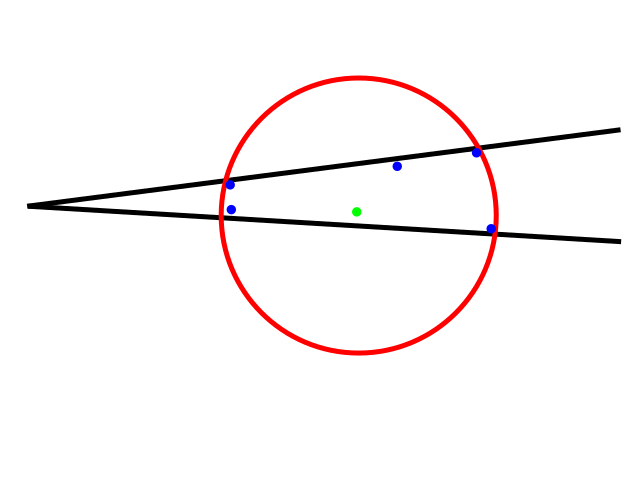
\includegraphics[scale=0.4]{images/bad_lambda.png}
    \caption{Limited sample point choice}
    \label{lspc}
\end{figure}

%As the number of dimensions grows the ratio of volume of the trust region intersect the feasible region to the feasible region can become smaller.

One way to handle this is to introduce a $\xi_{\text{cur}}$ which is allowed to decrease.
(Possibly, until a threshold is reached for maintaining a fixed $\Lambda$.)
If the new point does not improve the geometry of the set significantly, then there is no other point that would do better.
To test this, we introduce a constant $\delta_{\text{improv}}>0$ and require a new point to increase the current pivot by a factor greater than $\delta_{\text{improv}}$.
If the new point does not satisfy this test, we proceed with our current point and possibly decrease $\xi_{\text{cur}}$.
The new modified improvement algorithm is described in \cref{modified_model_improving_algorithm}:

\begin{algorithm}[H]
    \caption{Modified Model Improvement Algorithm}
    \label{modified_model_improving_algorithm}
    \begin{itemize}
        \item[\textbf{Step 0}] \textbf{(Initialization)} \\
            Initialize $i=1$.
            If the current sample set does not have $p$ points, repeat one of the current points. 
            Construct the Vandermonde matrix $V_{i,j} = \phi_j(\frac 1 {\Delta}(y^i - y^0))$.
            Initialize $0 < \ximin < \xi_{\text{desired}}$, $0 <\delta_{\text{improv}} < 1$,
            $  \xi_{\text{cur}} = \xi_{\text{desired}}$.
            
        \item[\textbf{Step 1}] \textbf{(Pivot)} \\
            Swap row $i$ with row $i_{\max} = \arg \max_{j|j\ge i} V_{j,i} $
        
        \item[\textbf{Step 2}] \textbf{(Check threshold)} \begin{itemize}
                \item[] If $|V_{i,i}| \ge \xi_{\text{cur}} $ then go to Step 3
                \item[] $ \hat y = \arg\max_{t \in \sampletrk \cap X} |\phi_i(t)|$
                \item[] If $\label{impossibly_poised} |\phi_i(\hat y)| < \ximin$ then \textbf{Stop}: the algorithm failed
                \item[] If $\xi_{\text{cur}} - |\phi_i(\hat y)| > \delta_{\text{improv}} \xi_{\text{cur}}$ then replace $V_{i,j}$ with $\phi_j(\hat y)$ and $\xi_{\text{cur}} \gets |\phi_i(\hat y)|$
            \end{itemize}
        
        \item[\textbf{Step 3}] \textbf{(LU)} \begin{itemize}
                \item[] Set $V_i \gets \frac{1}{V_{i,i}} V_i$
                \item[] Set $V_{,j} \gets V_{, j} - V_{i,j} V_{\bullet, i} \forall j=i \ldots p$
            \end{itemize}
            $i \gets i+1$
            Go to step 1 unless $i > p$
    \end{itemize}
\end{algorithm}

The \emph{ConstructTrustRegion} subroutine for this approach follows the prototype with $\sampletrk = \searchtrk = \feasiblek \cap \outertrk $.
As is usual, we may also wish to remove points larger than a certain radius from the current model center.
% If a lower bound $\kappa_{\phi}$ on the maximum value of each polynomial is known ahead of time, then the check on \cref{impossibly_poised} is not needed.
% That is, for a given set of linear constraints and largest trust region radius, it may be possible to calculate $\xi_{\text{min}} \le \kappa_{\phi} \le \max_{V}\max_{j}\max_{i}\|\phi_i(y^j)\|$.

%Another interesting approach we have not investigated is to decrease the size of the sample set when a new point cannot be computed.

%The analysis for this approach may be more difficult.




\subsection{Ellipsoidal Trust Region Approach}

If we adopt the ellipsoidal trust region approach to maintain a feasible inner trust region with a ``nice" shape we ensure of a stronger version of \cref{accuracy}.
Namely, we know from \cref{ellipsoidal_lambda} that 
\begin{align*}
    \|\mfk(x) - \nabla f(x) \| \le \kappa_g \Delta_{k} \quad \forall x \in \innertrk.
\end{align*}
If we also choose our trial point with \cref{search_a_little}, we have no guarantee of satisfying the efficiency condition \cref{efficiency} because $\dk$ is the outer trust region radius.
However, the model will likely be more accurate over this region.

%If bounds can be shown relating the model error of the inner trust region to the outer trust region, then we will satisfy \cref{accuracy}.
%In this case, classical methods ensure that $\|\nabla f(x^{(k)}) - \nabla m_f(x^{(k)})\| < \Delta_{inner} \le \dk$.

\subsubsection{Circular Trust Region}
The simplest approach to maintaining a feasible trust region is to set the inner trust region radius sufficiently small.
Within the \emph{ConstructTrustRegion} subroutine, this method sets the trust region radius to the distance to the closest constraint:
$\outertrk = B_2(\xk, \min\{\dk, \min_{i}\frac{|A_i\xk - b_i|}{\|A_i\|} \})$.
In practice, this does not work well as the radius can become too small to allow adequate progress.

Two general strategies were considered for addressing this issue as illustrated in \cref{options_basis}.
One option is to shift the center of the inner trust region as long as it remains within the outer trust region.
The second option is to elongate the trust region along the nearest constraint as discussed in the next section.
Of course, both of these can be done at the same time.


\begin{figure}[h]
    \centering
    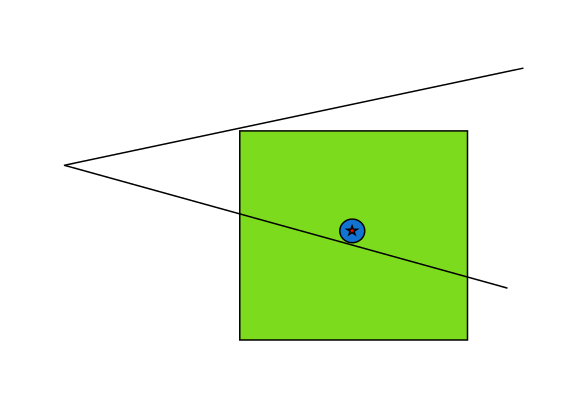
\includegraphics[width=200px]{images/small_circle.png}
    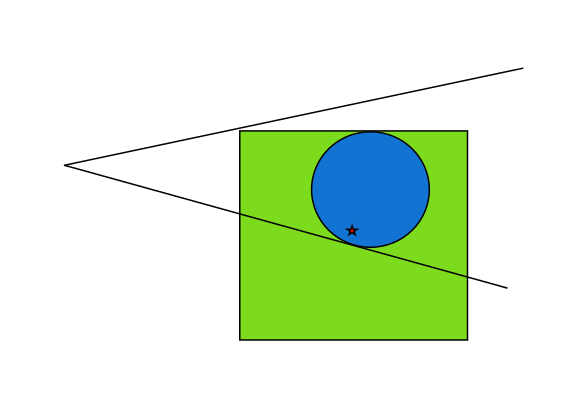
\includegraphics[width=200px]{images/shifted_center.png}
    \caption{When the current iterate is too close to a constraint, the circular trust region becomes too small. Shifting the trust region center helps remedy this. The star is the current iterate, the green is the outer trust region, and blue the inner.}
    \label{options_basis}
\end{figure}

\subsubsection{Ellipsoids}

In order to address this issue we considered using ellipsoidal trust regions.
Whereas the circle does not allow improvement when the current iterate lies along a constraint, an ellipsoid elongates along this constraint.
In figure \cref{ellipse_adv}, we have this type of iterate, but by using an ellipsoid we are still able to search towards the vertex of the feasible region.
\begin{figure}[h]
    \centering
    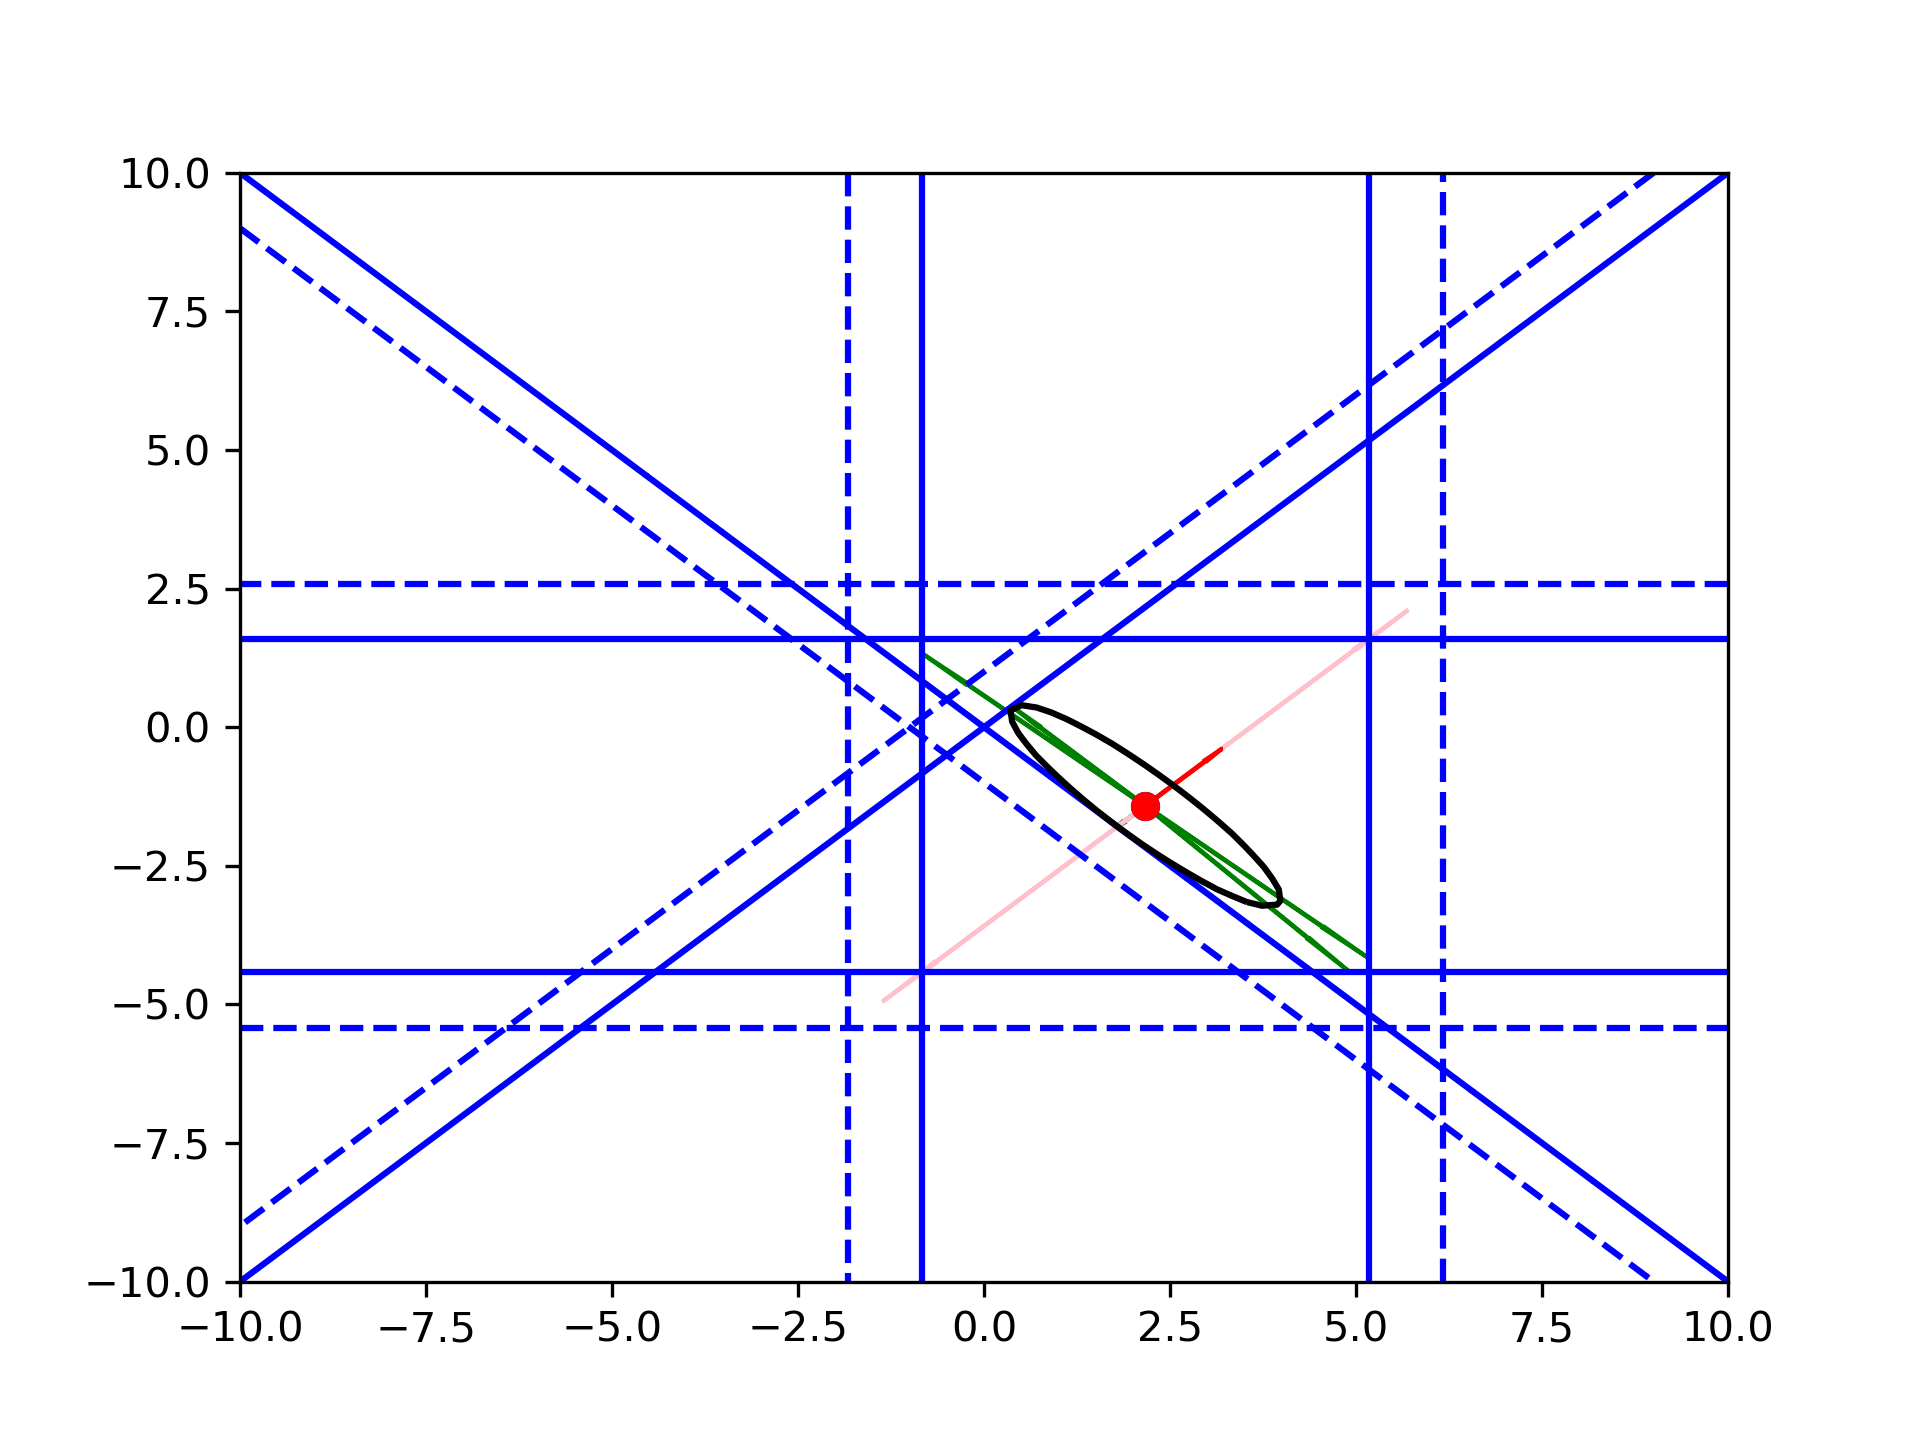
\includegraphics[scale=0.4]{images/advantage_of_ellipse_2.png}
    \caption{A nicer trust region}
    \label{ellipse_adv}
\end{figure}


More specifically, at iteration $k$, we choose a scaling factor $\pi^k$ and solve for an ellipsoid center $\mu^k$ and positive definite matrix $\qk$ to define an ellipsoid
$ \ellipsek = \{x \in \Rn \| \pi^k - \frac 1 2 (x - \mu^{k})^T\qk(x - \mu^{k}) \ge 0 \}$.
Of course, the simplest approach is to not change the center of the ellipsoid, but instead let $\mu^k = x^k$.


\subsubsection{Finding the Maximal $ \ellipsek $ Given $\mu^k$}

\label{ellipse_optimization}

Here, we first solve the problem of finding the maximum-volume ellipsoid given the center.
Later we perform a search over different centers of the ellipsoid.
%Because of this, we will first show how to find an ellipsoid with maximum volume given a fixed center.
We adopt a method similar to that described in \cite{Khachiyan1993}.
For now, we also let $\pi^k = 1$.

Given a polyhedron $P$ defined by an $m \times n$ matrix $A$, $P = \{ x \in \Rn\; | \;  Ax \le b \}$.
we wish to find the maximum-volume ellipsoid $E \subset P$ centered at a point $\mu \in P$.

Let $\bar{b} = b - A\mu$ and $d = x - \mu$ so that the polyhedron becomes
\begin{align*}
P = \{ \mu + d \in \Rn \; | \;  Ad \le \bar{b} \}
\end{align*}
Then, the ellipsoid can then be centered at zero, and defined by a symmetric positive definite matrix $Q \succ 0$:
\begin{align*}
E = \{ d \in \Rn \; | \; \frac 1 2 d^T Q d \le 1 \}.
\end{align*}
Our goal is to determine $Q$ to maximize the volume of $E$ such that $\mu + E \subset P$.
Define the auxiliary function $f(d) = \frac 1 2 d^T Q d$ so that $E = \{ d \in \Rn\; | \; f(d) \le 1 \}$.

Because $Q$ is positive definite, $f$ has a unique minimum on each hyper-plane $A_i d = b_i$.
Let this minimum be $d^{(i)} = \argmin_{A_id =\bar{b}_i} f(d)$ for $i=1,\ldots,m$.
By the first order optimality conditions, there exists a $\lambda \in \Rm$ such that
\begin{align*}
\nabla f(d^{(i)}) = Q d^{(i)} = \lambda_i A_i 
\Longrightarrow d^{(i)} = \lambda_i Q^{-1}A_i \quad \forall 1\le i\le m
\end{align*}
We also know that
\begin{align*}
A_i^T d^{(i)} = \bar{b_i} \Longrightarrow
A_i^T \lambda_i Q^{-1}A_i = \bar{b_i} \Longrightarrow
\lambda_i = \frac {\bar{b_i}}{A_i^T  Q^{-1}A_i}
\end{align*}
so that
\begin{align*}
d^{(i)} = \lambda_i Q^{-1}A_i = \frac {\bar{b_i}}{A_i^T  Q^{-1}A_i}  Q^{-1}A_i \quad \forall 1\le i\le m.
\end{align*}

Because $E \subset P$, we also know that $f(d^{(i)}) \ge 1$ for each $i$. Thus,
\begin{align*}
\frac 1 2 (d^{(i)})^{T} Q d^{(i)} \ge 1 \\
\Longrightarrow \frac 1 2 \bigg(\frac {\bar{b}_i}{A_i^T  Q^{-1}A_i}  Q^{-1}A_i\bigg)^{T} Q \frac {\bar{b}_i}{A_i^T  Q^{-1}A_i}  Q^{-1}A_i \ge 1 \\
\Longrightarrow \frac 1 2 \frac {1}{A_i^T  Q^{-1}A_i}  \bar{b_i} A_i^T Q^{-1} Q \frac {\bar{b_i}}{A_i^T  Q^{-1}A_i}  Q^{-1}A_i \ge 1 \\
\Longrightarrow \frac 1 2 \frac {1}{A_i^T  Q^{-1}A_i}  \frac {\bar{b_i}^2}{A_i^T  Q^{-1}A_i}  A_i^T Q^{-1}A_i \ge 1 \\
\Longrightarrow \frac 1 2  \frac {\bar{b_i}^2}{A_i^T  Q^{-1}A_i} \ge 1 \\
\Longrightarrow \frac 1 2 \bar{b_i}^2\ge A_i^T  Q^{-1}A_i \\
\Longrightarrow A_i^T  Q^{-1}A_i \le \frac 1 2 \bar{b_i}^2
\end{align*}

Because the volume of the ellipsoid is proportional to the determinant of $Q^{-1}$, the maximal ellipsoid is defined by

\begin{align*}
Q = V(\mu) = \sup_{Q \succeq 0} \det(Q^{-1}) \\
s.t. \quad A_i^T Q^{-1} A_i \le \frac 1 2 \bar{b_i}^2
\end{align*}


% This problem includes a maximization of a determinant.
% In order to ensure that the trust region goes to zero, we must also ensure that the maximum eigenvalue of the matrix is bounded.
% Thus, for some bound $M^k$ we define $Q^k$ as
%  & eig(Q)_i \le M^k & \forall i \in \mathcal I \cup \mathcal E \\
% 
% After shifting the center to $\mu$, this problem takes the form:
% 
% \begin{center}
% \begin{align}
% \label{ellipse_1}
% \qk = V(\mu^k) = \sup_{Q \succ 0} & \det(Q^{-1}) & \\
%   & {A^k}_i^T Q^{-1} {A^k}_i \ge \frac 1 2 (b^k - A^k\mu^{k})^T(b^k - A^k \mu^{k}) & \nonumber
% \end{align}
% \end{center}


\subsubsection{Poisedness over Ellipsoidal Trust Regions}
\label{ellipsoidal_lambda}

% TODO: Find a better reference
It is possible to show $\Lambda$-poisedness for an ellipsoidal region with a change of variables to the ball centered around the origin.
We wish to construct a model for $f(x)$ in the ellipsoidal region
$\ellipsek = \{x \in \Rn | (x - c)^T\qk(x - c) \le 1\}$ for some symmetric, positive definite
$\qk \in \mathbb R^{n\times n}$ and some center $c \in \Rn$.
We can give $\qk$ its eigen-decomposition $\qk = L D^2 L^T$, where $L^TL = I$ and $D$ is a diagonal matrix with nonnegative entries.
If we let $\delta = \max_{x\in \ellipsek}\|x-c\|$, then the transformation $T(x) = \delta DL^T(x - c)$ maps $ \ellipsek $ to the $\delta$ ball $\{u = T(x) \in \Rn \; | \; \|u\| \le \delta\}$.
Conversely, $ T^{-1}(u) = \frac 1 {\delta} LD^{-1}u + c$ maps the $\delta$ ball to the ellipsoidal region $ \ellipsek $.

% \cref{fully_quadratic}

\begin{theorem}
\label{shifted_ellipsoid}
Let $T$ and $\delta$ be as defined above, and let $\hat m_f(u)$ be a model of the shifted objective $\hat f(u) = f(T^{-1}(u))$ in the $\delta$ ball such that
there exist constants $\kappa_{ef}, \kappa_{eg}, \kappa_{eh} > 0$ such that for all $\{u \in R^n | \;\|u\| \le \delta \}$, we have
% for all $u \in B(0 ; \delta)$ we have the following error bounds:
\begin{align*}
|\hat m_f(u) - \hat f(u)| \le \kappa_{ef} \delta^3\\
\|\nabla \hat m_f(u) - \nabla \hat f(u)\| \le \kappa_{eg}\delta^2\\
\|\nabla^2 \hat m_f(u) - \nabla^2 \hat f(u)\| \le \kappa_{eh}\delta.
\end{align*}

Then, with
\begin{align*}
\kappa_{ef}' = \kappa_{ef} \\
\kappa_{eg}' = \kappa_{eg}\sqrt{\kappa(\qk)} \\
\kappa_{eh}' = \kappa_{eh}\kappa(\qk),
\end{align*}
we have that for all $x \in \ellipsek$,
the model function $m_f(x) = \hat m_f(T(x))$ will satisfy
\begin{align*}
| m(x) - f(x)| \le \kappa_{ef}'\delta^3 \\
\|\nabla  m(x) - \nabla  f(x)\| \le \kappa_{eg}'\delta^2 \\
\|\nabla^2 m(x) - \nabla^2 f(x)\| \le \kappa_{eh}'\delta.
\end{align*}
\end{theorem}

\begin{proof}

% Notice  that for all $x\in \ellipsek$ we have 
% \begin{align*}
% \|x-c\| \le \delta \\
% \|T(x-c)\| \le \delta \\
% \end{align*}
% so that $\frac{\|T(x-c)\|}{\|x-c\|} \le 

We know that $\delta = \frac 1 {\sqrt{\lambda_{\text{min}}(\qk)}} = \frac 1 {\min_{i} D_{i, i}}$.
This means,
\begin{align*}
\kappa(\qk) = \kappa(D^2) = \frac{\max_{i}D_{i,i}^2}{\min_{i}D_{i,i}^2} = \delta^2 \max_{i}D_{i,i}^2 = \delta^2 \|D\|^2 \\
\|D\| = \frac 1 {\delta} \sqrt{\kappa(\qk)} \le \frac{\kappa_{\lambda}}{\delta}.
\end{align*}

Also, $\delta \le \dk$ as the ellipse is constructed within the outer trust region.
\color{red}
% For all $x \in  \ellipsek$, we have that
% \begin{align*}
% \delta^2 \lambda_{\text{min}}(Q) \le \lambda_{\text{min}}(Q) (x-c)^T(x-c) \le (x-c)^TQ(x-c) \le 1 \\
% \lambda_{\text{max}} x^T x\le 1 \\
% \|x\|^2 \le \frac 1 {\lambda_{\text{max}}} \\
% \|x\| \le \frac 1 {\sqrt{\lambda_{\text{max}}}} \\
% \end{align*}


% Notice that because $\ellipsek \subset T(\ellipsek)$ and $\|T(x-c)\| = \|x-c\|$ along the major axis, we must have $\lambda_{\text{min}}(T) = 1$.
% This means that $\delta min_{i} D_{i,i} = 1 \Longrightarrow \delta = \frac{1}{\min_{i}D_{i,i}}$.
% Because the major axis of the ellipse is preserved, we also
% smallest eigenvalue of $T$ is $1$.
% \begin{align*}
% \kappa(Q) = \kappa(D^2) = \frac{\max_{i}D_{i,i}^2}{\min_{i}D_{i,i}^2} \ge \delta^2 \max_{i}D_{i,i}^2 = \delta^2\|D\|^2
% \end{align*}

\color{black}

Then, we have for all $\{u = T(x) \; | \; \|u\| \le \delta \} \Leftrightarrow x \in \ellipsek$

%\Leftrightarrow \{x = T^{-1}(u) \; | \; \|T^{-1}(u)\| \le 1 \} 

% \begin{align*}
% \delta^2\kappa(Q) = \|D\|
% \end{align*}
% smallest eigenvalue of t is one
% 

\begin{align*}
 | m_f(x) - f(x)| = |\hat m(u) - \hat f(u)| \le \kappa_{ef}'\dk^3.
\end{align*}

Similarily, for the gradient we find:

\begin{align*}
\| \nabla m_f(x) - \nabla f(x)\| = \delta\left\|DL^T\left(\nabla\hat m_f(u) - \nabla \hat f(u)\right)\right\| \le \delta \|DL^T\|\|\nabla \hat m_f(u) - \nabla \hat f(u)\| \le \sqrt{\kappa(\qk)}\kappa_{eg} \delta^2 \\
\end{align*}

% \begin{align*}
% \|\nabla \hat m_f(u) - \nabla \hat f(u)\| \le \Lambda \kappa_{eg} \delta^2\\
% \|\nabla ( m_f(T^{-1}(u))) - \nabla ( f(T^{-1}(u)))\| \le \Lambda \kappa_{eg} \delta^2\\
% \|\nabla \left( m_f(\frac 1 {\delta} D^{-T}L^Tu + c)\right) - \nabla \left( f(\frac 1 {\delta} D^{-T}L^Tu + c)\right)\| \le \Lambda \kappa_{eg} \delta^2\\
% \|\frac 1 {\delta} LD^{-1} \nabla  m_f(\frac 1 {\delta} D^{-T}L^Tu + c) - \frac 1 {\delta} LD^{-1} \nabla  f(\frac 1 {\delta} D^{-T}L^Tu + c)\| \le \Lambda \kappa_{eg} \delta^2\\
% \|LD^{-1} \left(\nabla  m_f(x) - \nabla  f(x)\right)\| \le \Lambda \kappa_{eg} \delta^3\\
% \|DL^T\|\|LD^{-1} \left(\nabla  m_f(x) - \nabla  f(x)\right)\| \le \Lambda \kappa_{eg} \delta^3 \left(\frac {\kappa_{\lambda}} {\delta}\right) \\
% \|\nabla  m(x) - \nabla  f(x)\| \le \Lambda \kappa_{eg}' \delta^2 \le \Lambda \kappa_{eg}' \dk^2. \\
% \end{align*}
Finally, we show that for the Hessian:

\begin{align*}
\| \nabla^2 m_f(x) - \nabla^2 f(x)\| = \delta^2\left\|DL^T\left(\nabla\hat m_f(u) - \nabla \hat f(u)\right)LD^T\right\| \le \delta^2 \|D\|^2\|\nabla \hat m_f(u) - \nabla \hat f(u)\| \le \kappa(\qk)\kappa_{eh} \delta \\
\end{align*}

% \begin{align*}
% \|\nabla^2 \hat m_f(u) - \nabla^2 \hat f(u)\| \le \Lambda \kappa_{eh} \delta\\
% \|\nabla^2 \left(m_f(\frac 1 {\delta} D^{-T}L^Tu + c)\right) - \nabla^2 \left(f(\frac 1 {\delta} D^{-T}L^Tu + c)\right)\| \le \Lambda \kappa_{eh} \delta\\
% \frac 1 {\delta^2} \|LD^{-1} \nabla^2 m_f(\frac 1 {\delta} D^{-T}L^Tu + c) D^{-T}L^T - LD^{-1} \nabla^2 f(\frac 1 {\delta} D^{-T}L^Tu + c) D^{-T}L^T\| \le \Lambda \kappa_{eh} \delta\\
% \|LD^{-1} \left(\nabla^2 m_f(x) - \nabla^2 f(x) \right) D^{-T}L^T\| \le \Lambda \kappa_{eh} \delta^3 \\
% \|DL^T\|\|LD^{-1} \left(\nabla^2 m_f(x) - \nabla^2 f(x) \right) D^{-T}L^T\|\|LD\| \le \Lambda \kappa_{eh}\delta^3\left(\frac {1}{\delta^2}\kappa(\qk)\right)  \\
% \|\nabla^2 m_f(x) - \nabla^2 f(x)\| \le \Lambda \kappa_{eh}' \delta \le \Lambda \kappa_{eh}' \dk\\
% \end{align*}




% \begin{align*}
% \min_{i}D_{i,i} = \frac{\dk }{\text{length longest axis of ellipse}} \\
% \frac{1}{\min_{i}D_{i,i}} = \frac{\text{length longest axis of ellipse}}{\dk } \le 1\\
% \frac{1}{\min_{i}D_{i,i}^2} = \bigg(\frac{\text{length longest axis of ellipse}}{\dk }\bigg)^2 \le 1\\
% \kappa(Q) = \max_i D_{i,i}^2 \bigg(\frac{\text{length longest axis of ellipse}}{\dk }\bigg)^2 \le \max_i D_{i,i}^2\\
% \kappa(Q) = \frac{\max_{i}D_{i,i}^2}{\min_{i}D_{i,i}^2} = \|D\|\delta \le \kappa_{\lambda} \\
% \|DL^T\| \le \frac{\kappa_{\lambda}}{\delta}\\
% \end{align*}

\end{proof}

This shows that in order to have strongly quadratic model functions, we need only bound the condition number of $\qk$.
For the purposes of a convergence proof, we need only satisfy the weaker accuracy condition \cref{accuracy}.
Notice that in practice the model functions do not need to be mapped to the $\delta$ ball, because $\Lambda$-poisedness is scale invariant \cite{DUMMY:intro_book}.
The implications of this proof are discussed futher in the convergence discussion \cref{convergence_discussion}.

% After constructing a $\Lambda$-poised set on the unit ball, we can construct a shifted model function
%  that accurately models a shifted objective  over a ball.
% Namely, from , we know that for some constants , we have that for all :
 

% Letting $\delta = \frac 1 {\min_i D_{i,i}^2}$, and forcing the condition number of $Q$ to be less than or equal to a fixed constant $\kappa_{\lambda}$, we see that
%\color{red}
%We notice that the length of the largest axis of the ellipsoid is bounded by $\dk$, so that $\min_{i}D_{i,i}^2 \le \dk$.
%\color{black}

%Given a constant $\kappa_{\lambda} > 0$, we force 
%so that


% right hand sides are one
% little delta is the max|x-c|, x \in  E
% T(x) = little delta DL^T(x - c)
% smallest eigenvalue of t is one
% \kappa(little delta ^2 Q) = \|D\|
% mapping onto little delta



%These new constants $\kappa_{ef}', \kappa_{eg}', \kappa_{eh}'$ depend only on the largest eigenvalue of $Q$.

\subsubsection{Ellipsoid Choices}

There are a number of issues to be solved to define this ellipsoid:
\begin{itemize}
\item How do we ensure that $\xk \in \ellipsek $?
\item How do we choose $\ellipsek$ in such a way that it does not limit travel along a decent direction?
\item How do we choose the center of the ellipsoid $\mu^k$?
\end{itemize}

% \item How do we choose $\ellipsek$ to make the  ellipsoid as large as possible while ensuring that $ \ellipsek \subset \outertrk \cap \feasiblek $?

If $\xk \not \in \searchtrk $, the ellipse may not even contain a point with any reduction.
Thus, we have implemented a few ways of ensuring the current iterate is within the search trust region.
This can be done by either of the following two options:
\begin{itemize}
\item Adding a constraint to the ellipsoid problem to include the original point.
\item Expand the size of the ellipsoid.
\end{itemize}

%IMAGES GO HERE

\paragraph{Adding a constraint.}
In order to include the original point as a constraint, we add a constraint to the definition of the ellipsoid of the following form:
$$ \pi^k - \frac 1 2 (x^k - \mu^{k})^T\qk(x^k - \mu^{k}) \ge 0. $$
Constraints of this nature make finding the ellipsoid much more expensive.
This is because the optimization problem we construct uses ${\qk}^{-1}$ as decision variables, so that constraints in terms of $\qk$ must model matrix inversion.

\paragraph{Increase the size.}
An alternative is to scale $\qk$ by a constant.
We use the scaling factor $\pi^k$ defined by

$$\pi^{(k)} = \max \{1, \frac 1 {2} (x^{k} - \mu^{k})^T \qk (x^{k} - \mu^{k})^T \}$$

and let the ellipsoid be:
$$\ellipsek = \{x \in \Rn | 1 - \frac 1 {2\pi^k} (x - \mu^{k})^T \qk (x - \mu^{k}) \ge 0\} $$
However, this means that in general $\ellipsek \not \subset \feasiblek$ so that the trust region subproblem must contain constraints for both the ellipsoid and the feasible region: $\searchtrk = \ellipsek \cap \domain$.

To help mitigate the second issue, we maximize the volume of the ellipsoid.
However, the choice of ellipsoid center can still limit travel along a decent direction.
Choosing the best center is the topic of the next section.\

% 
% \paragraph{One theoretical concern}
% 
% %The are some other concerns to be considered while defining the ellipsoid.
% % While choosing $\ellipsek$, 
% 
% %We also want consecutive ellipsoid to share volume, in order to avoid evaluating as many points as possible.
% %(So far, we have been re-evaluating the set of trial points each iteration.)
% 
% 
% Lastly, when $\ellipsek \subset \feasiblek$, we may not be able find a second order solution.
% This is becase the ellipsoid can only be tangent to the constraint, and some decent paths may be missed.
% In \cref{fbns}, the red line represents a path in the feasible region that is always decreasing.
% However, if the trust regions decrease without intersecting this path, the algorithm will not be aware of this descent path.
% However, scaling the trust region to the outer green radius may allow the algorithm to ensure global convergence to second order critical points.
% 
% \begin{figure}[h]
%     \centering
%     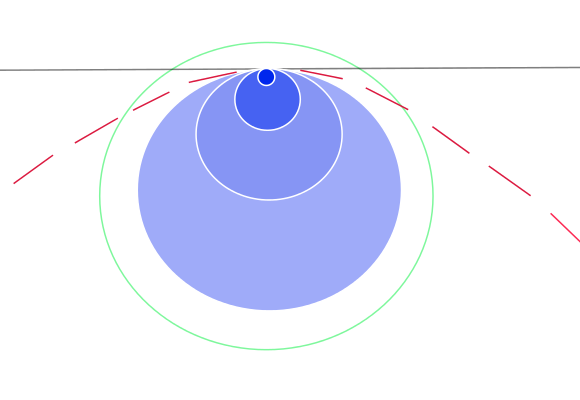
\includegraphics[width=200px]{images/second_order_critical_point.png}
%     \caption{Potential issue with a second order critical point.}
%     \label{fbns}
% \end{figure}
% 


% Finally, we have the problem of computing the ellipsoid once given a suitable definition.


\subsection{Searches for the Center}

We consider several different approaches for determining the trust region center $\mu^k$.
In this case, our \emph{ConstructTrustRegion} subroutine searches over multiple centers of the ellipsoid, however it may not need to construct the model functions for each until it has found a desirable ellipsoid.




%For now, we maximize the volume of $E_k$, .

%For now, we have simply used the heurstic $H(E_k) \to \text{Vol}(E_k)$.
%Given a huristic $H : \innertrk \to \Theta$, where $\Theta$ is a set of comparable elements, the \emph{ConstructTrustRegion} routine follows the following template:

%\begin{algorithm}[H]
%    \caption{Heuristic Search}
%    \label{heuristic_search}
%    \begin{itemize}
%        \item[] \textbf{Initialization} Initialize $T_{\text{best}} = \emptyset$, $\theta_{\text{best}} = H(T_{\text{best}})$
%            
%        \item[] \textbf{For all $\mu \in$ search space do:} \begin{itemize}
%                \item[] $T_{\text{trial}} \gets \arg\max_{E_k \text{centered at} \mu} \text{Vol}(E_k)$
%                \item[] $\theta_{\text{trial}} = H(T_{\text{trial}})$
%                \item[] If $\theta_{\text{trial}} \le \theta_{\text{best}}$ then continue
%                \item[] $T_{\text{best}} = T_{\text{trial}}$
%                \item[] $\theta_{\text{best}} = \theta_{\text{trial}}$
%            \end{itemize}
%    \end{itemize}
%\end{algorithm}


\subsubsection{Search Everything}

One approach is to search all possible centers within $ \feasiblek \cap \outertrk $.
That is, we solve:
$$\mu^k = \sup_{\mu \in \feasiblek \cap \outertrk} V(\mu)$$
where $V(\mu)$ is the volume of the ellipsoid defined in \cref{ellipse_1}.
%The search within the \emph{ConstructTrustRegion} is allowed to go anywhere within $ \feasiblek \cap \outertrk$.
This has the advantage that it captures much of the feasible region.
However, one problem with this search is that it can force the trust region away from the desired direction.
Notice that in \cref{ellipse_runs_away}, although the ellipsoid found has larger volume than before being shifted, this ellipsoid contains points farther from the corner containing the minimizer.

\begin{figure}[h]
    \centering
    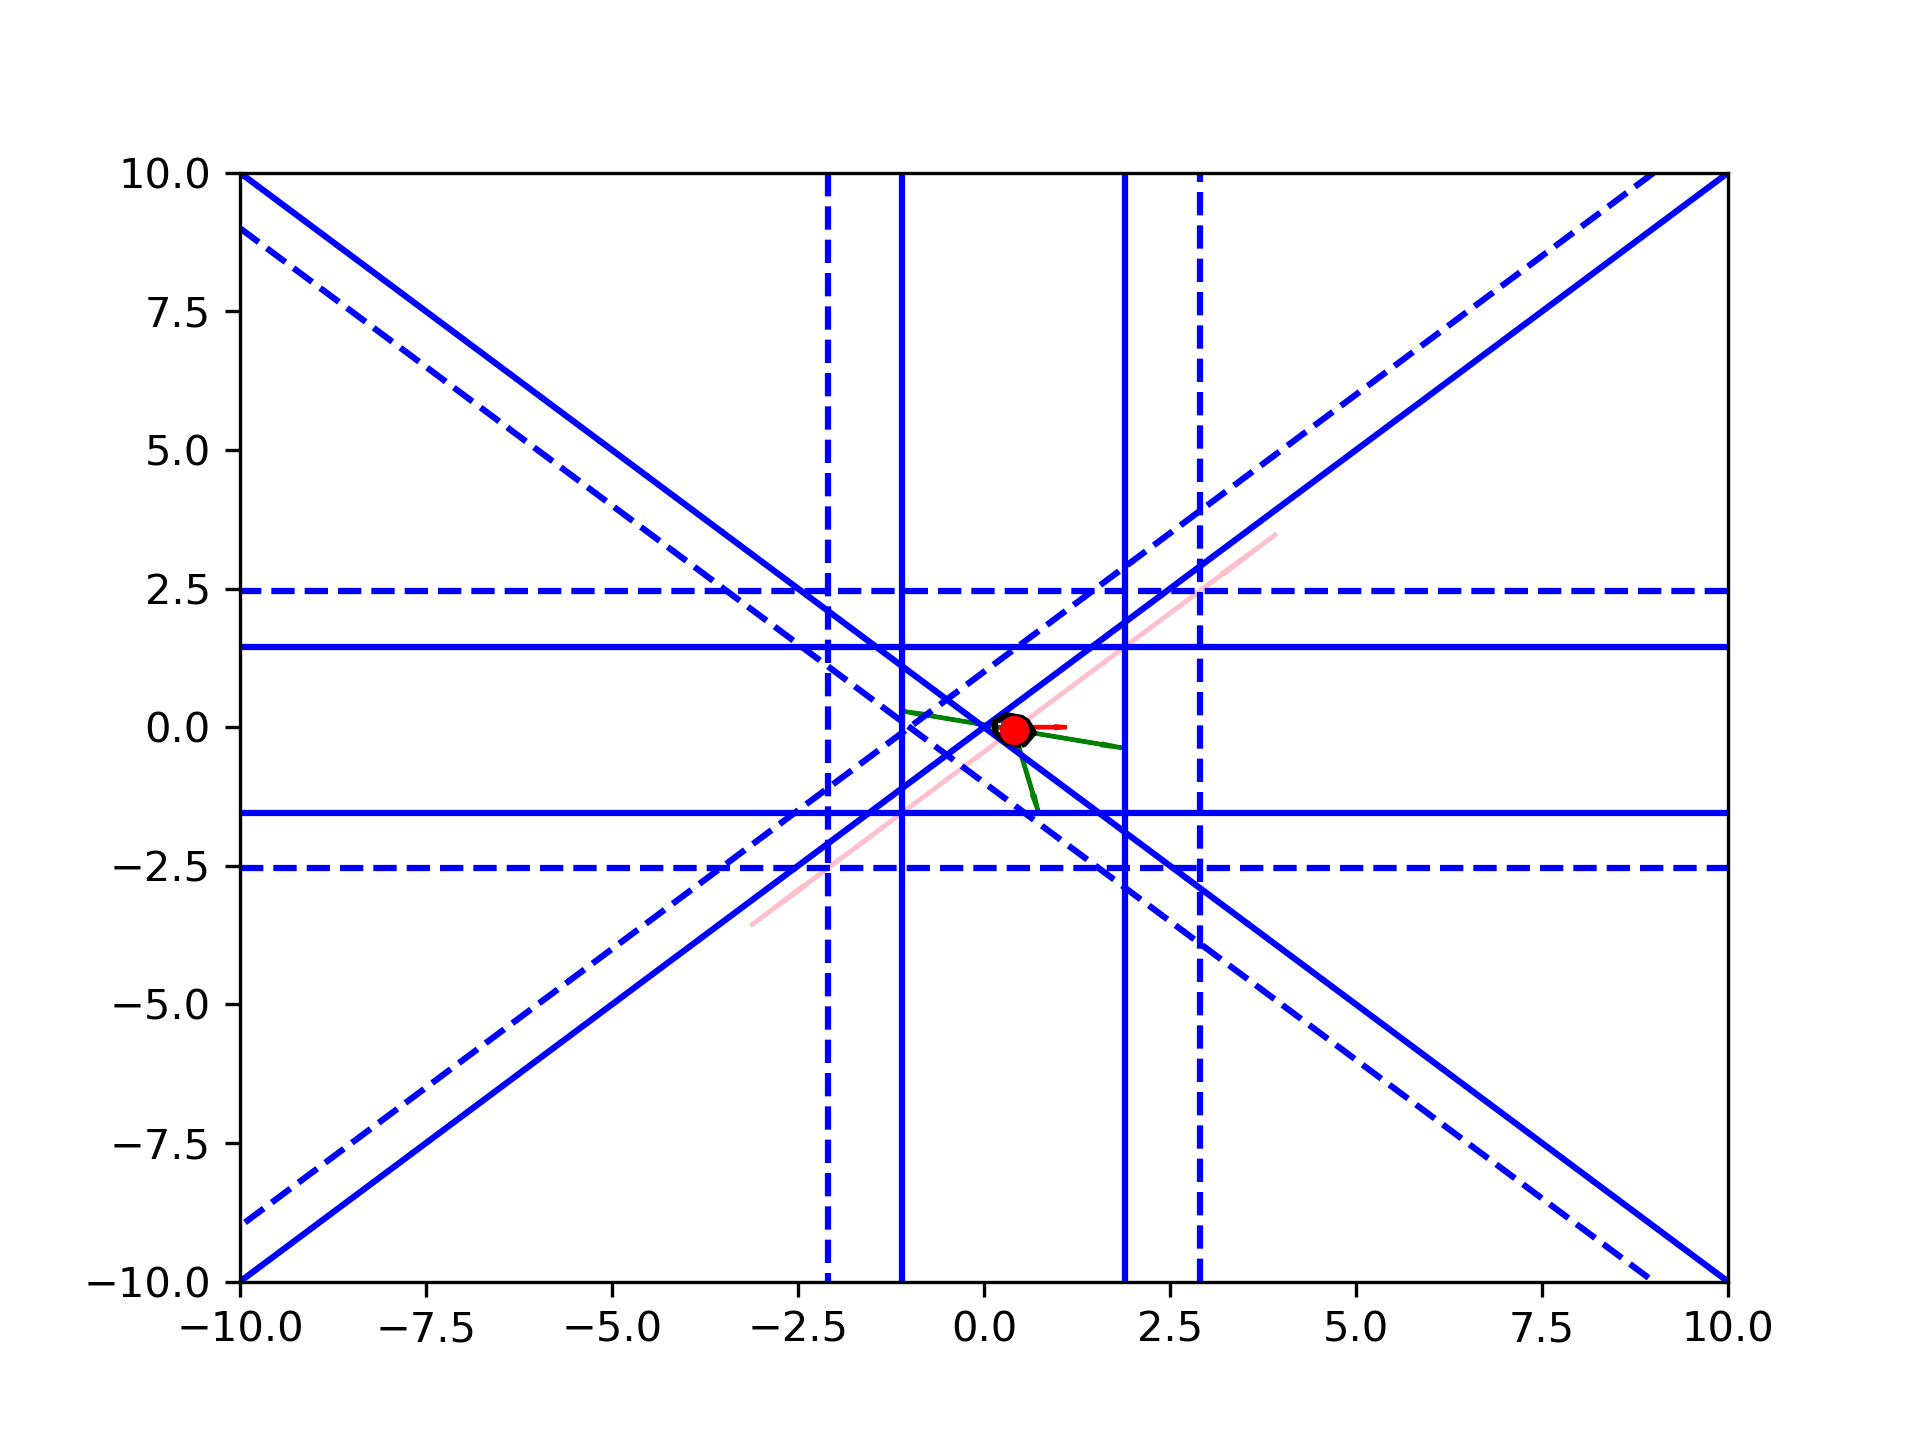
\includegraphics[scale=0.4]{images/everything_runs_1.png}
    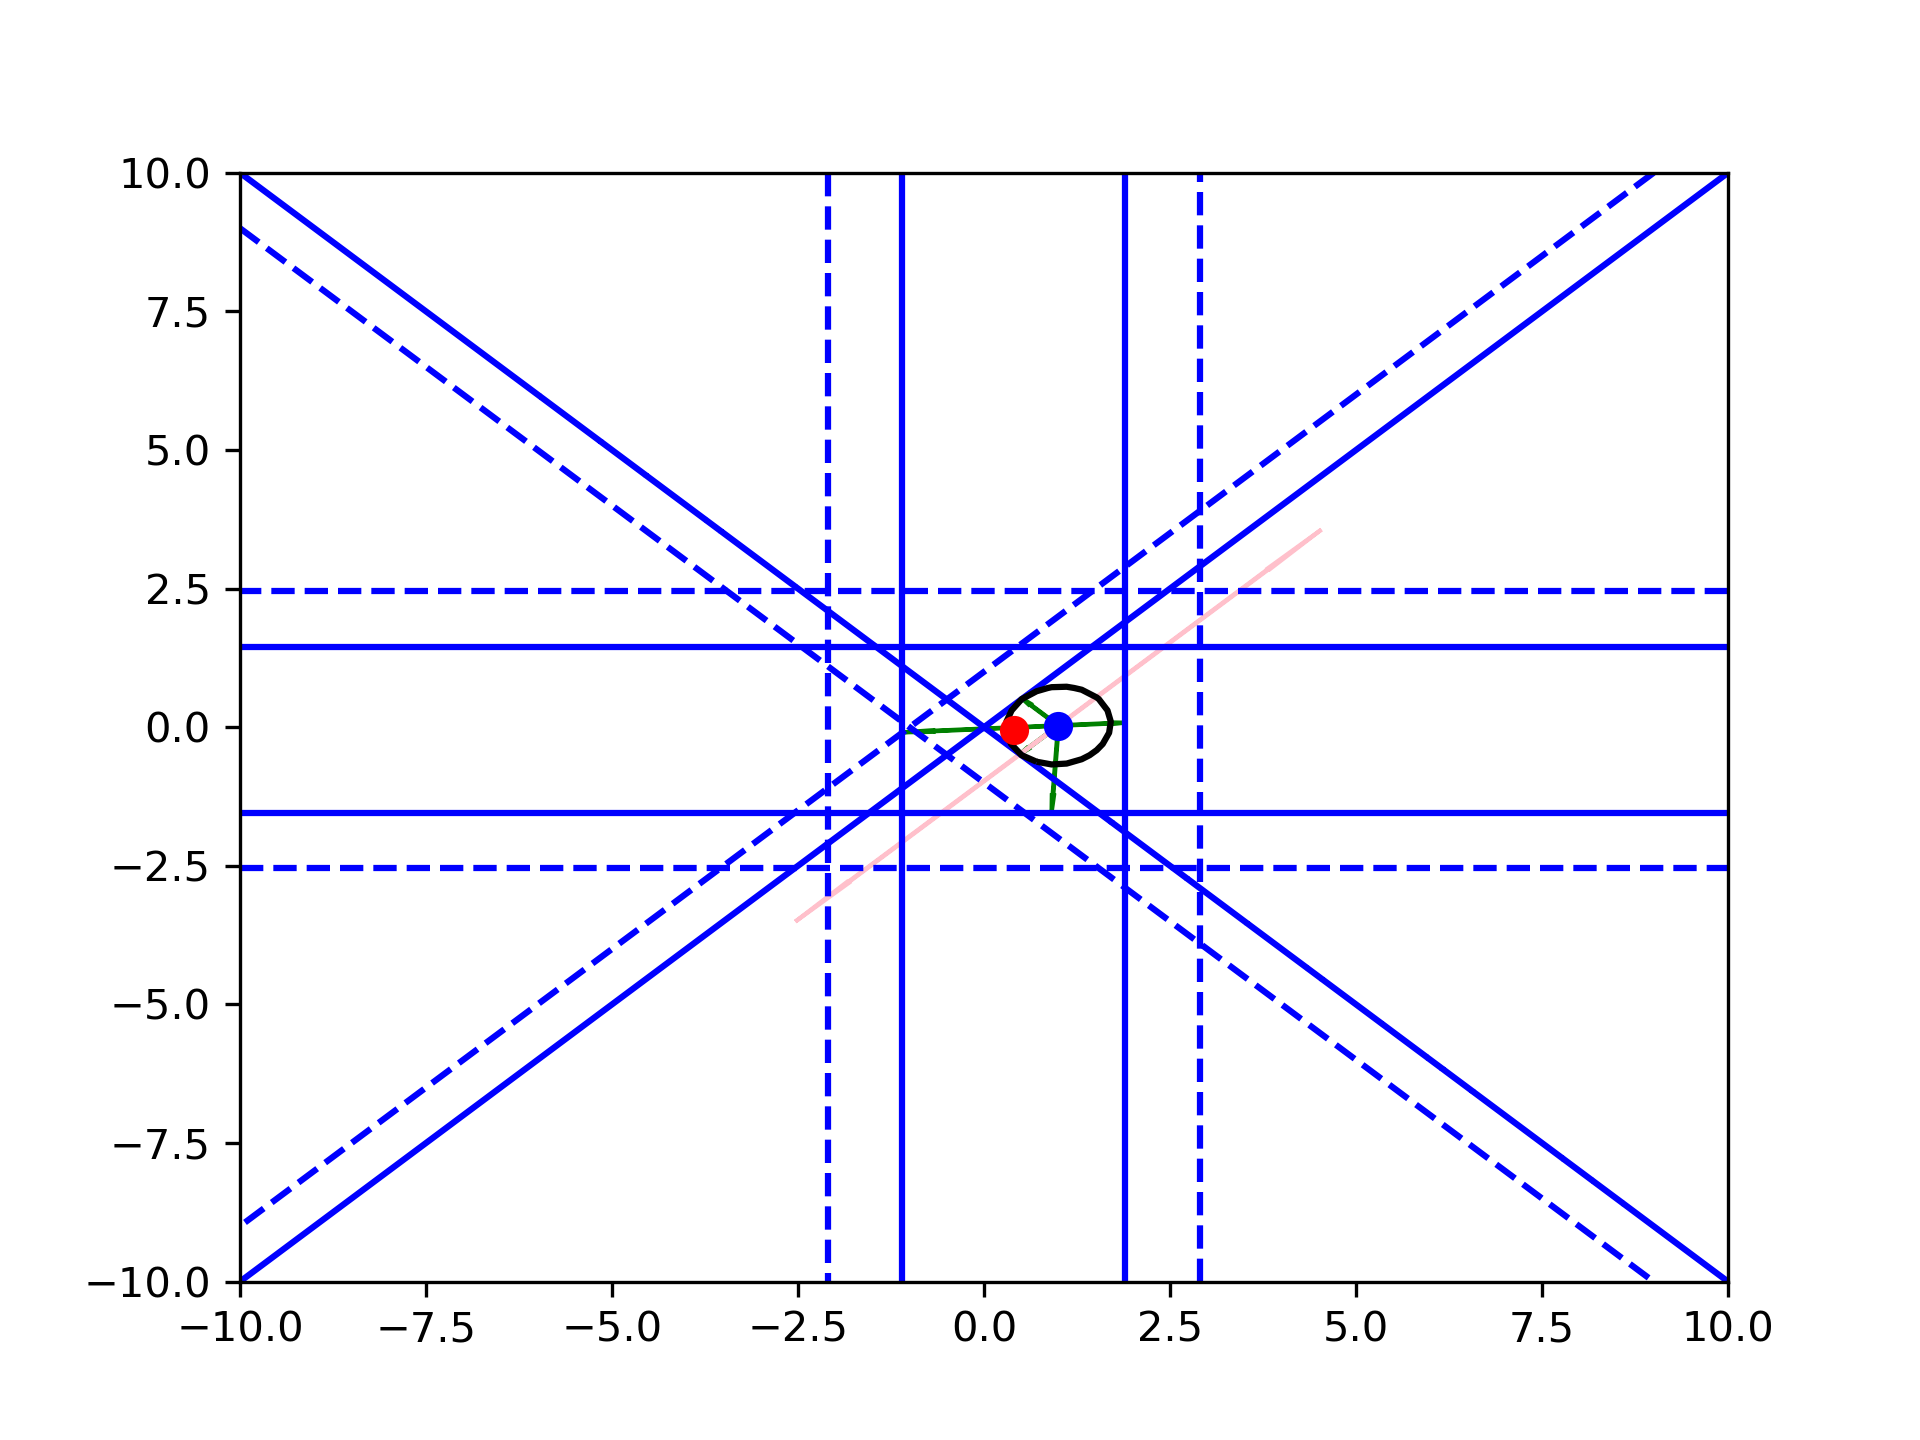
\includegraphics[scale=0.4]{images/everything_runs_2.png}
    \caption{Searching $\feasiblek$}
    \label{ellipse_runs_away}
\end{figure}


One attempt to fix this problem is by limiting the search direction for the center of the ellipsoid.


\subsubsection{Line Searches}
Although $\mfk$'s minimizer over $\outertrk$  can appear anywhere, there are some reasons for expecting it to be at a ``vertex."
If it lies in the interior, there is little need for using constrained approaches once near the solution.

%The ellipsoid with maximum volume, however, tends to lead $ \sampletrk $ away from vertices.
One way of trying to ensure a feasible direction towards a vertex, while still allowing a larger volume ellipsoid, is by limiting the search for the new center to lie on line segments starting at the current iterate $\xk$.

For example, our first attempt was to simply search a line directed orthogonally away from the closest constraint.
This has obvious problems as shown in \cref{first_line_search}, as we should avoid letting the new center get closer to another constraint:

\begin{figure}[h]
    \centering
    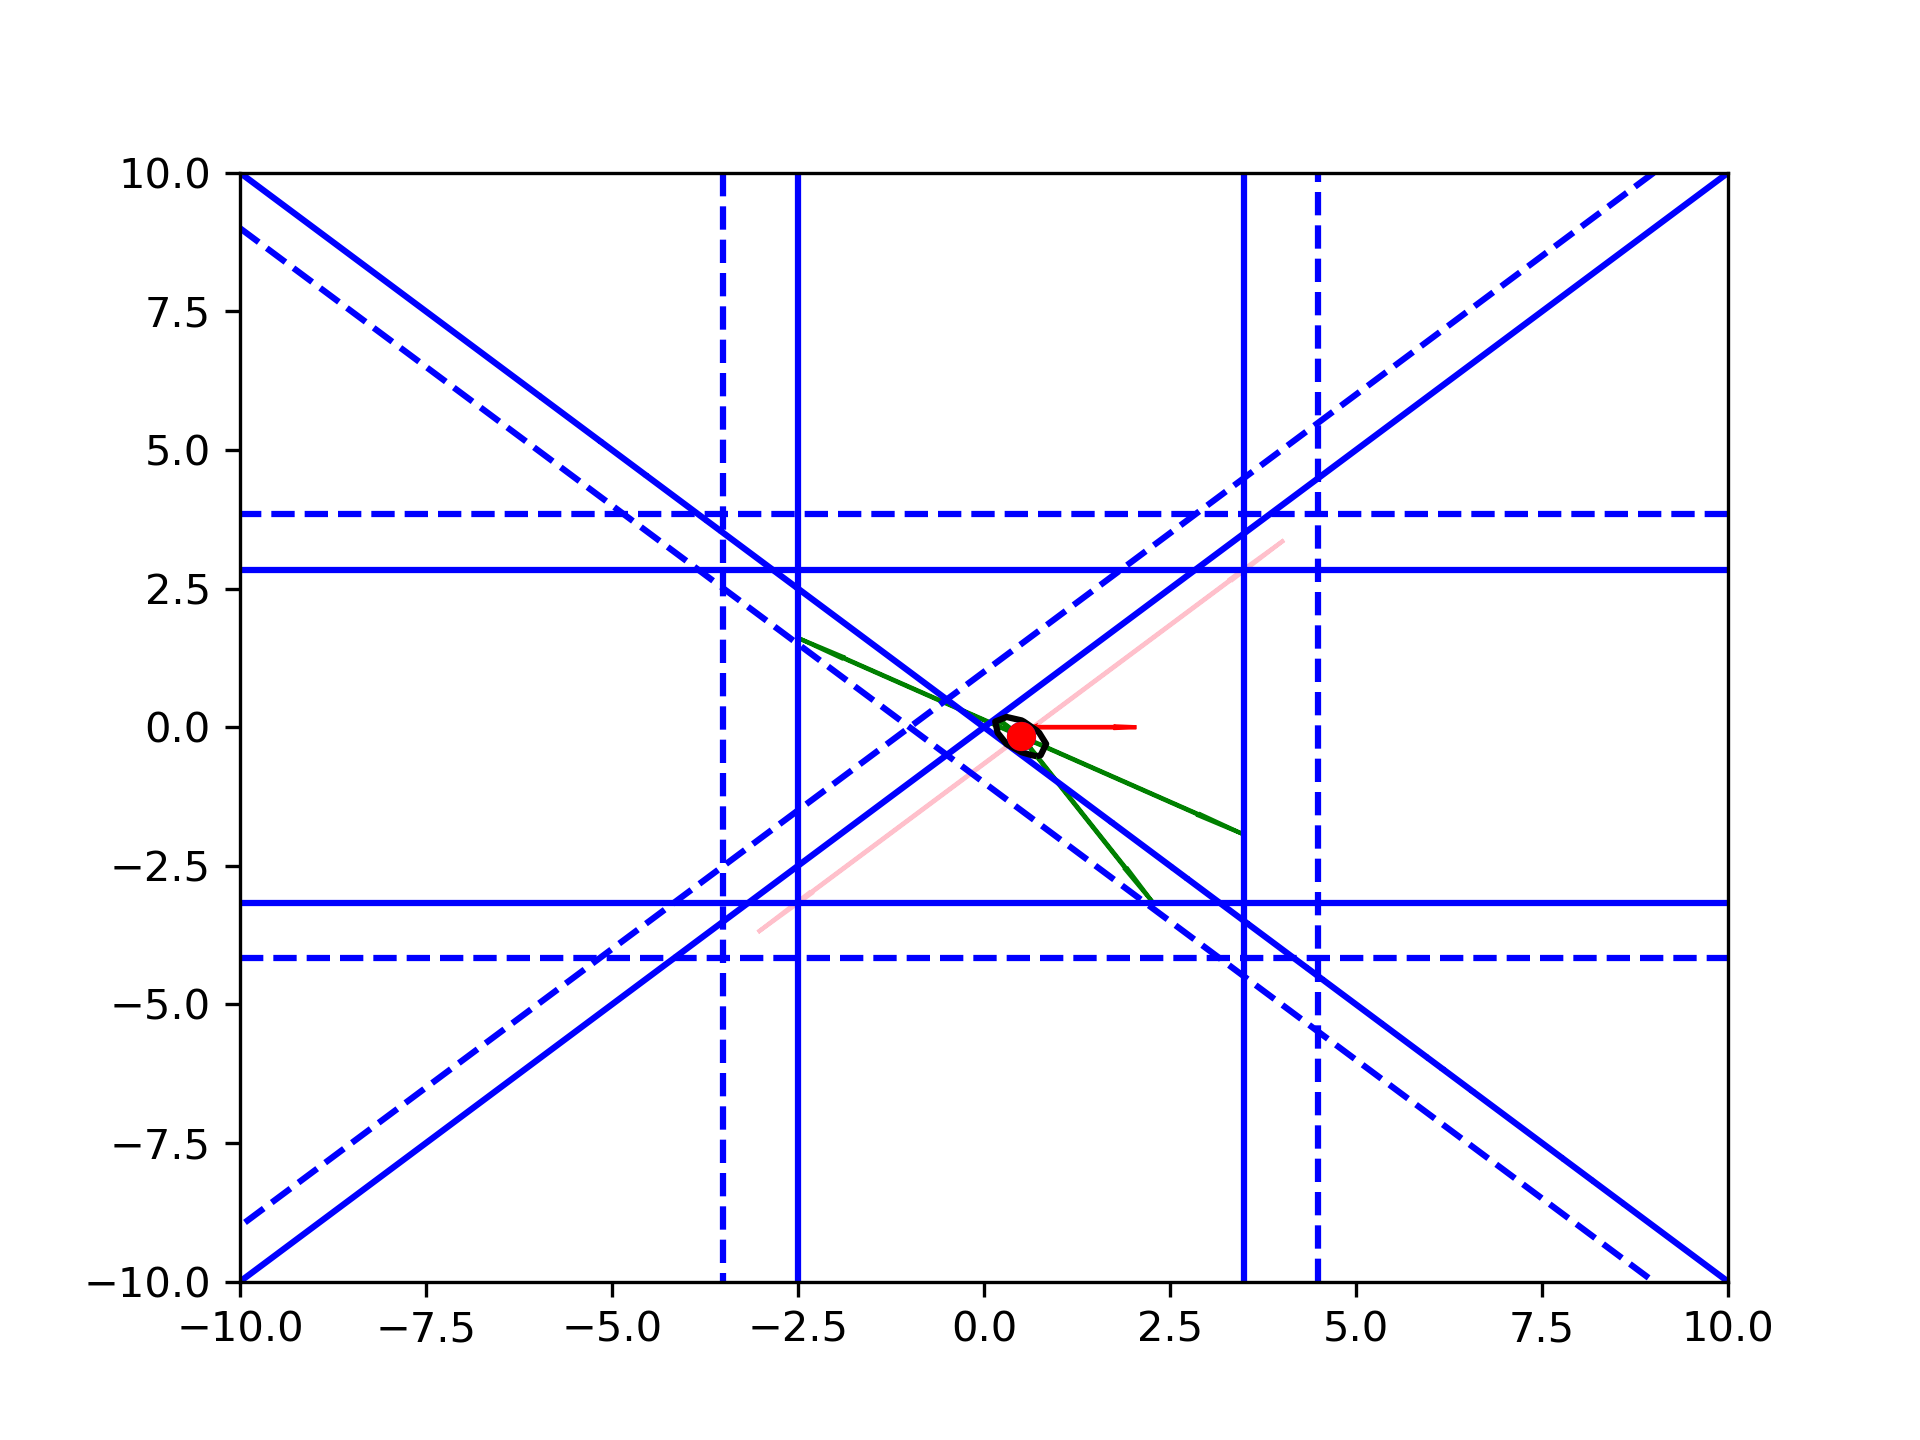
\includegraphics[scale=0.4]{images/line_1.png}
    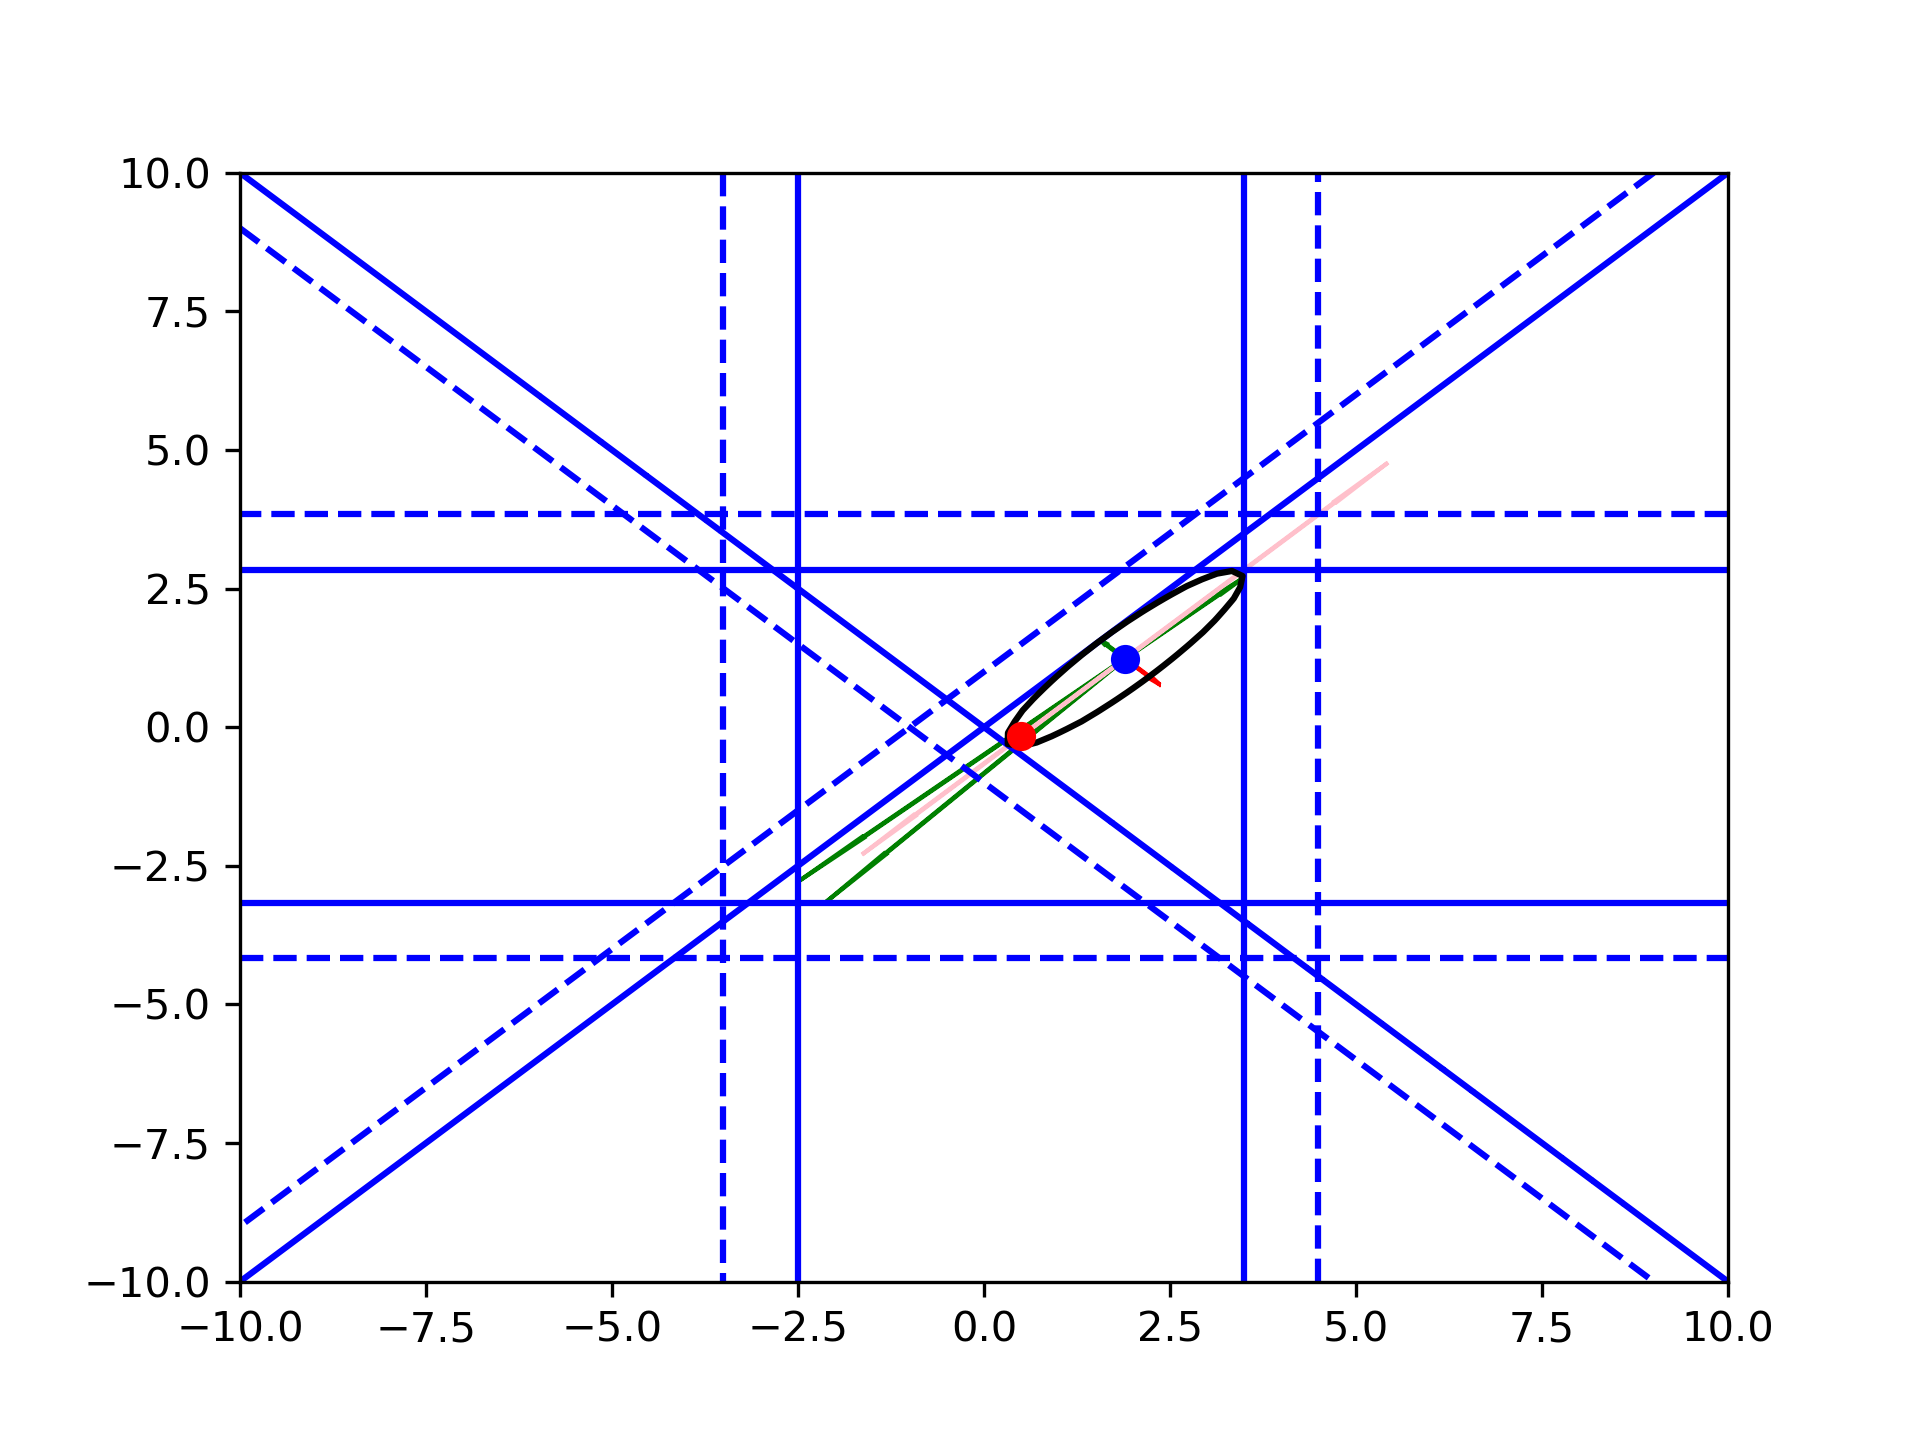
\includegraphics[scale=0.4]{images/line_2.png}
    \caption{Line searches}
    \label{first_line_search}
\end{figure}


For a given distance $d$, let the indices $i$ for which $\frac {|A_i x - b|}{\|A_i\|} \le d$


To fix this, we break the search space within the \emph{ConstructrustRegion} subroutine into segments based on the nearest constraints.
The algorithm works by choosing a set of up to $n_{\text{points}}$ points $s_1, s_2, \ldots, s_{n_{\text{points}}}$ that are each equidistant to a subset of the constraint's faces.
The center search then considers points along the line segments between these points.
% Namely, it starts at the current iterate and travels along a ray away from all the closest constraints until it reaches a point equidistant to yet another constraint.

More precisely, the first point is chosen to be the current iterate: $s_1 = \xk$.
The algorithm then repeats the following process for $i$ from $1$ to $n_{\text{points}}$.
First, compute the set of nearest constraints, where the distance from a point $x$ to a constraint $A_i$ is given by $d(A_i, x) = \frac {|A_i x - b|}{\|A_i\|}$.
While finding the next point $s_{i+1}$, let  $A_E$ be a normalized array of the equidistant faces $\{\frac{A_i}{\|A_i\|} | d(A_i, s_i) = \min_j d(A_j, s_i), i = 1, 2, \ldots, m\}$ and $b_E$ be the rows' corresponding values of $b$.
All other faces are called the remaining faces, and construct the matrix $A_R$ and vector $b_R$.
It then finds a search direction $p  = r{A_E}^T$ as a linear combination of the normal vectors to the equidistant faces.
%When the constraint violation of $s_i$ is non-zero, this search ray can be found by finding the point that doubles the current slack ${A_E}s_i-{b_E}$.
%This is given by $r{A_E}^T$ where $r$ solves the linear system ${A_E}(s_i + r{A_E}^T) - b_E = 2 ({A_E}n_i - b_E)$.
%If the current violation is zero, then the right hand side can be set to a vector of all ones to ensure that all slacks violations are the same: $A_E(s_i + r{A_E}^T) - b_E = 1$.
This search ray can be found by setting the slack to each equidistant face to a vector of all ones: $A_E(s_i + r{A_E}^T) - b_E = 1$.
We can travel along this ray until we reach a point that is the same distance to a remaining face.
Specifically, we can travel by 
\begin{align}
t = \argmin_j {\frac{d({A_E}_0, s_i) - d({A_R}_j, s_i)}{ {A_R}_j - d({A_E}_0) p} | ({A_R}_j - d({A_E}_0) p > 0 }. 
\end{align}

We can then set $s_{i+1} = s_{i} + t p$.

Of course, $n_{\text{points}}$ must be less than or equal to $n + 1$ in order for this to be defined.
Also, the algorithm must stop early if $A_E$ contains parallel faces.

% if we let $\nabla \modelconstrainti(\xk) = A_i$ be the $i$th row of $A$, then we define the distance from a search point $s$ so the $i$th constraint to be


This means that we can define a class of searches that each limit the number of line segments to search $n_{\text{points}}$.

In figure \cref{line_can_run}, the red line shows the line segments equidistant their closest constraints.
Notice that with two line segments, the algorithm can already choose new centers further from the vertex.

% TODO: REPLACE PICTURES
\begin{figure}[h]
    \centering
    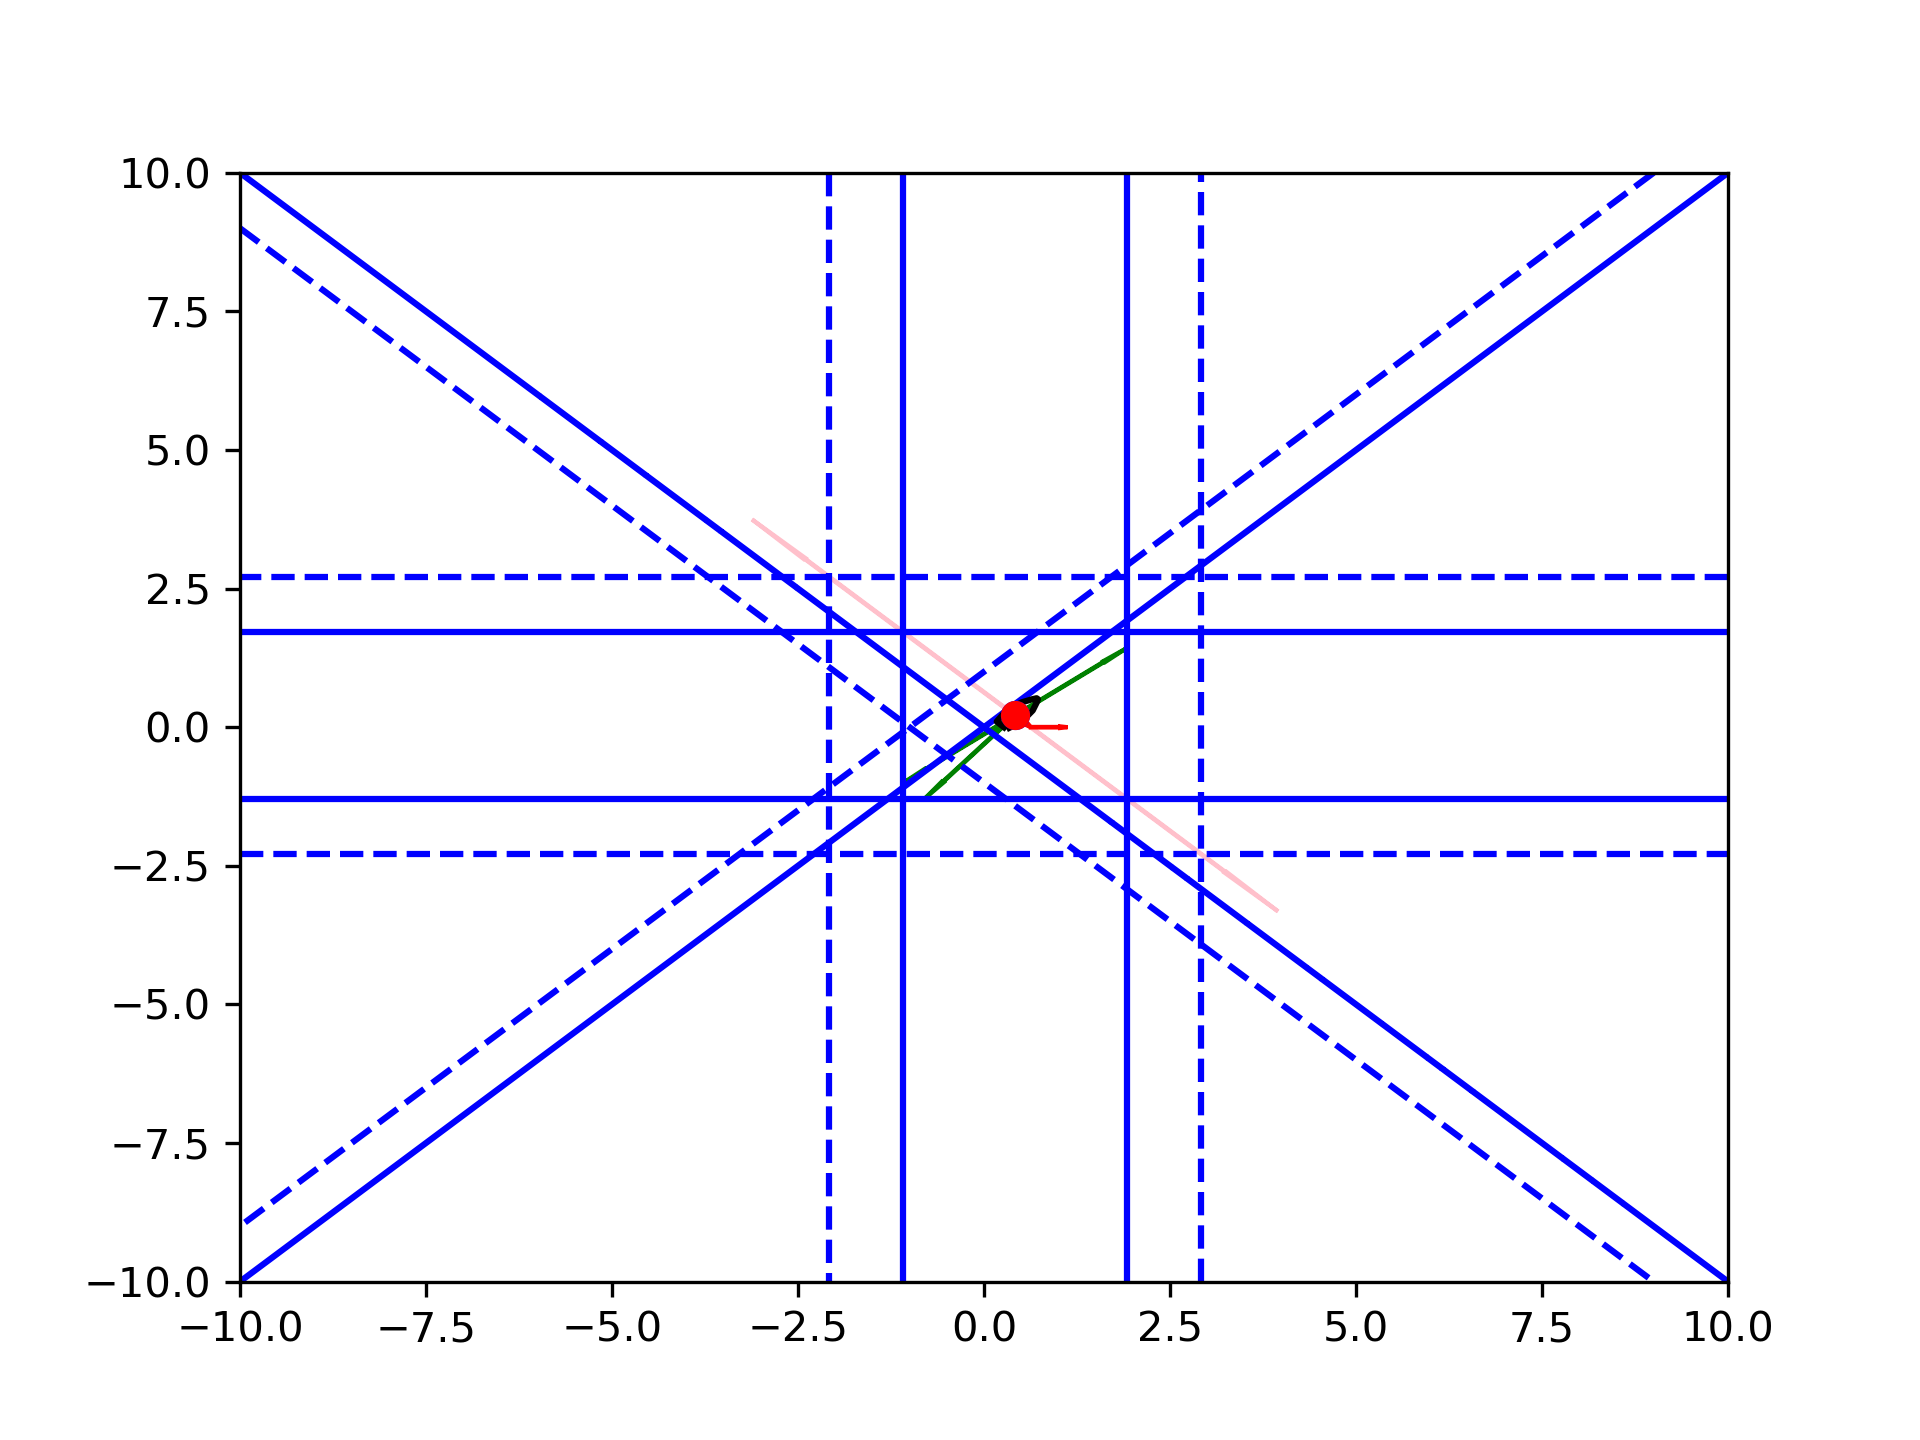
\includegraphics[scale=0.4]{images/run_away_1.png}
    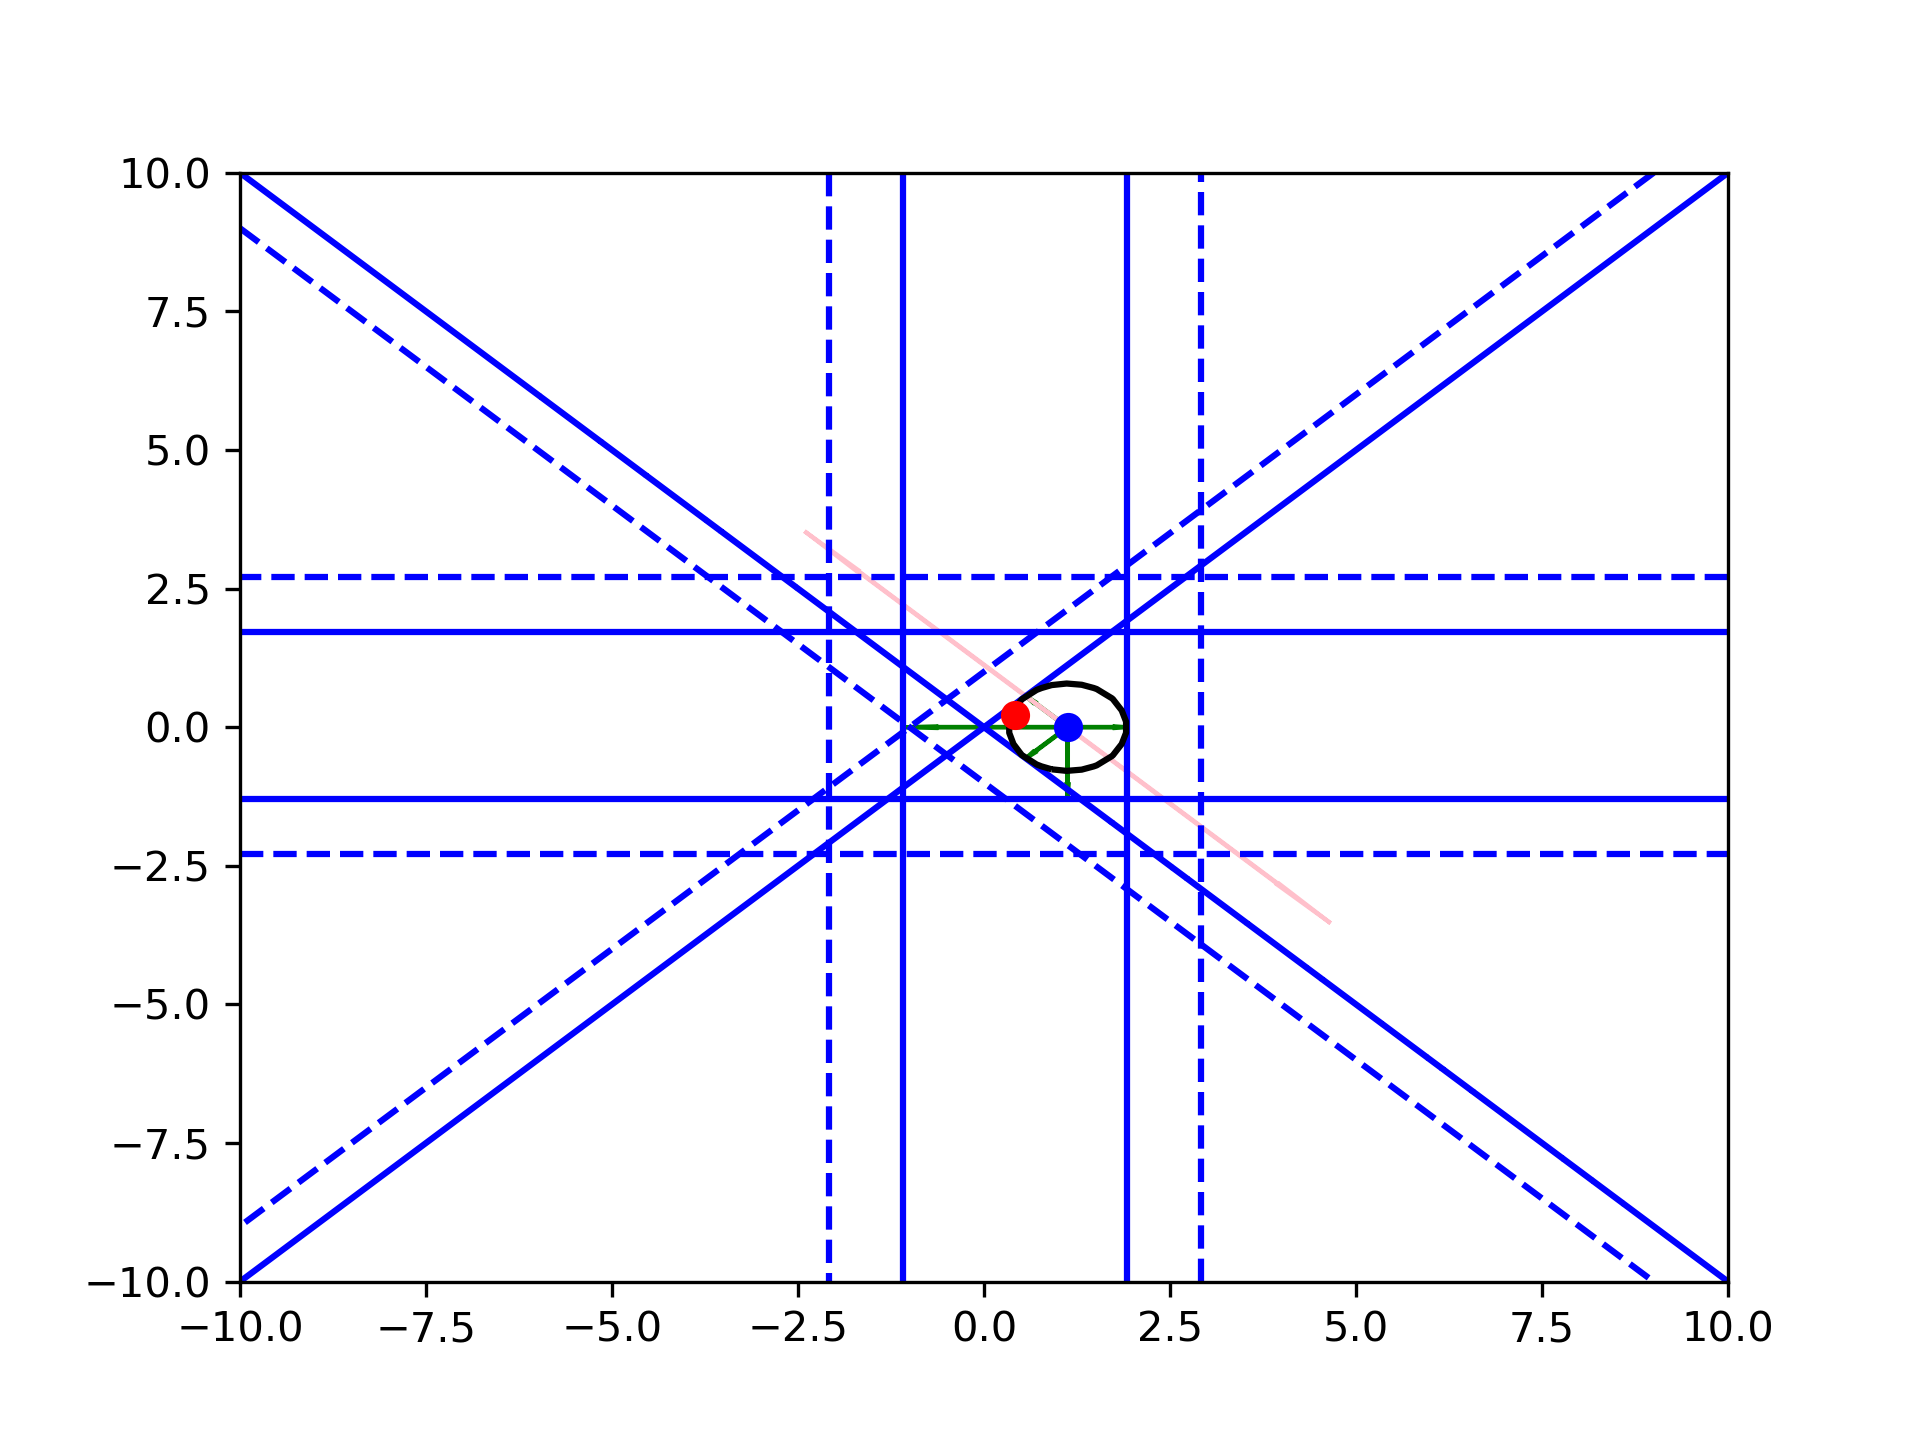
\includegraphics[scale=0.4]{images/run_away_2.png}
    \caption{Ellipse runs away from the optimizer}
    \label{line_can_run}
\end{figure}




\section{Convergence Discussion}

Here, we show convergence for one version of \cref{constrained_dfo}.
Namely, we choose to satisfy \cref{bluepill} and let $\sampletrk$ have an ellipsoidal shape as described in \cref{sample_region_choices}. 
Also, we will select \cref{search_a_lot} as discussed in \cref{search_region_choices}: namely, $\searchtrk = \outertrk \cap \feasible$.
To do this, we require the following assumptions.

\begin{assumption}
The function $f$ is differentiable and its gradient $\nabla f$ is Lipchitz continuous with constant $L_{g} > 0$ in $\domain$.
\begin{align}
\label{lipschitz}
\|\nabla f(x) - \nabla f(y)\| \le L \|x - y\| \quad \forall x, y \in \domain
\end{align}
\end{assumption}

\begin{assumption}
\label{for_fully_quadratic}
The function $f$ has Lipschitz continuous hessian with constant $L_h > 0$ in $\domain$.
\begin{align}
\label{lipschitz_hessian}
\|\nabla^2 f(x) - \nabla^2 f(y)\| \le L_h \|x - y\| \quad \forall x, y \in \domain
\end{align}
\end{assumption}

\begin{assumption}
The function $f$ is bounded below over $\domain$.
\begin{align}
\label{lower_bound}
f(x) \ge \fmin \quad \forall x \in \domain
\end{align}
\end{assumption}


\begin{assumption}
\label{uniformly_bounded_hessians_of_mf}
The Hessian's of $\mfk$ are uniformly bounded at each iterate. That is, there exists a constant $\beta \ge 1$ such that $\|\nabla^2 \mfk(\xk)\| \le \beta - 1$ for all $k \ge 0$
\end{assumption}

Lastly, the accuracy condition \cref{accuracy} must be satisfied.
\begin{assumption}
\label{accuracy_assumption}
There exists a constant $\delta_g$ such that $\|\nabla m_k(\xk) - \nabla f(\xk)\| \le \delta_g \dk$ for all $k \ge 0$.
\end{assumption}
This is dealth with in \cref{satisfying_accuracy}.


Also, we add some assumptions of our own.
\begin{assumption}
\label{interior_point}
There exists a point $\bar x$ within the interior of the feasible region: $A\bar x < b$.
\end{assumption}

\label{convergence_discussion}

If the tolerances $\tau_{\chi} = 0$ and $\tau_{\Delta} = 0$ are set to zero, the algorithm presented here is a particular implementation of the algorithm presented in \cite{doi:10.1080/10556788.2015.1026968}.
This means we only need to satisfy the requirements detailed in their convergence analysis.


\subsection{Algorithm Assumptions}
For your convenience, we duplicate the assumptions found in \cite{doi:10.1080/10556788.2015.1026968}.
Firstly, they assume that the algorithm satisfies an efficiency condition \cref{efficiency}.

\begin{itemize}
\item[$H_0$] The efficiency condition \cref{efficiency} is satisfied.
\item[$H_1$] The function $f$ is differentiable and its gradient $\nabla f$ is Lipchitz continuous with constant $L > 0$ in $\domain$.
\item[$H_2$] The function $f$ is bounded below over $\domain$.
\item[$H_3$] The matrices $H_k$ are uniformly bounded. That is, there exists a constant $\beta \ge 1$ such that $\|\nabla^2 \mfk\| \le \beta - 1$ for all $k \ge 0$.
\item[$H_4$] There exists a constant $\delta_g$ such that $\|\nabla m_k(\xk) - \nabla f(\xk)\| \le \delta_g \dk$ for all $k \ge 0$.
\end{itemize}

$H_0$ can be satisfied within our algorithm by selecting the Generalized Cauchy Point \cite{Conn:2000:TM:357813} to solve the trust region subproblem.
Notice that $H_1$, $H_2$, and $H_3$  are kept as hypothesis within our algorithm.

The only assumption not yet dealth with is $H_4$, which is the topic of \cref{satisfying_accuracy}.
However, first we show a way of using a more straightforward version of $H_3$ in \cref{simpler_h3}.

\subsection{Satisfying these assumptions}
From here on, we will assume that the iterates $\xk$ are chosen according to \cref{constrained_dfo}.
This implies that each of the sample points used to construct $\mfk$ are output of \cref{model_improving_algorithm}.


XXXX
Because of \cref{lipschitz_hessian} and \cref{lipschitz_gradient}, $f$ satisfies \cref{introduction_3_1} and hence the assumptions for \cref{quadratic_errors}.
Notice that because $\kappa_f$, $\kappa_g$, $\kappa_h$ only depend on $p$, $L_h$, and $\Lambda$, these values do not depend on the iteration $k$:
using the same tolerance $\xi_{\text{min}}$ is used within \cref{model_improving_algorithm} implies a bound on $\Lambda$.
XXXX
 
, and therefore $\mfk$ satisfies the requirements for \cref{quadratic_errors}.
is a fully quadratic model over $B_{\infty}(\xk, \dk)$.
Because the constraints are linear, we will let $G$ be the $m \times n$ normalized gradient of the constraints $g$ be the scaled constraint values at $0$, so that
\begin{align}
\|G_i\| = 1\;\forall 1\le i\le m \\
\feasiblek = \feasible = \{x \in \Rn | c(x) \le 0 \Leftrightarrow G x \le g \} \label{define_g}
\end{align}
Remember that $\feasible \subset \domain$.

\subsubsection{More simple $H_3$}
\label{simpler_h3}
First, we show that \cref{uniformly_bounded_hessians_of_f} can be used instead of \cref{uniformly_bounded_hessians_of_mf} under some restrictions.
Namely, for this to be true, we also first assume:
\begin{assumption}
\label{delta_max}
There exists a $\Delta_{\text{max}} > 0$ such that $\dk \le \Delta_{\text{max}}$ for all $k \ge 0$.
\end{assumption}

With this modest assumption, we can make the assumptions more straightforward by replacing \cref{uniformly_bounded_hessians_of_mf} with \cref{uniformly_bounded_hessians_of_f}:

\begin{assumption}
\label{uniformly_bounded_hessians_of_f}
The Hessian's of $f$ are uniformly bounded at each iterate. That is, there exists a constant $\beta \ge 1$ such that $\|\nabla^2 f\| \le \beta - 1$ for all $k \ge 0$
\end{assumption}


This is the result of the following lemma:
\begin{lemma}
\label{replacing_h3}
Assume that \cref{uniformly_bounded_hessians_of_f},  \cref{lipschitz_hessian}, \cref{delta_max} are satisfied and that each $k \in \naturals$, $\mfk$ satisfies of $f$ over $B_{\infty}(\xk, \dk)$  as in \cref{quadratic_errors}.
Then \cref{uniformly_bounded_hessians_of_mf} is also satisfied.
\end{lemma}

\begin{proof}
Let $\beta_1 \ge 1$ be such that for all $k \ge 0$:
\begin{align*}
\|\nabla^2 f(\xk) \| \le \beta_1 - 1
\end{align*}
% \cref{model_improving_algorithm},
Because $\mfk$ are fully quadratic, we know that \cref{error_in_hessian} is satisfied.
Combining this with \cref{delta_max} we see that
\begin{align*}
\|\nabla^2 f(\xk) - \nabla^2 m_f(\xk) \| \le \kappa_{h} \dk \le \kappa_{h} \Delta_{\text{max}}
\end{align*}
Defining $\beta_2 = \kappa_{h} \Delta_{\text{max}} + \beta_1 \ge 1$, we see that
\begin{align*}
\|\nabla^2 m_{f}(\xk) \| \le \|\nabla^2 m_{f}(\xk) - \nabla^2 f(\xk)  \| + \|\nabla^2 f(\xk) \|  \le \beta_2 - 1 .
\end{align*}
\end{proof}

% For any $x \in \feasible$, we have that the set of gradients of active constraints is linearly independent. That is, the vectors $\{\nabla c_i(x) |  \forall i \in \activei(x)\}$ is linearly independent.


\subsubsection{Satisfying \cref{accuracy_assumption}}
\label{satisfying_accuracy}
The only remaining assumption is the accuracy condition \cref{accuracy_assumption}.

As discussed in \cref{ellipsoidal_lambda}, we know that if the condition number of $\qk$ is bounded, we will have a well poised model.
However, we must also ensure that we are always able to find a feasible ellipsoid.
Although it is not always possible to find a feasible ellipsoid that contains the current iterate,
we can find a feasible ellipsoid that only needs to be scaled by a constant to do so.
% It is shown in \cite{Billups_Larson_2013} that a lambda poised set over a sphere remains lambda poised over a larger sphere (with a larger lambda).


% \activei_k = \activei(\xk) \\


\new

Let $\mathcal S \subseteq \{1, \ldots, m\}$ be arbitrary.
We define
\begin{align}
\activei(x) = \{1 \le i \le m | c_i(x) = 0 \Leftrightarrow Gx = g \} \label{active_indices} \\
\alphaone (\mathcal S) = \begin{cases}
\argmax_{\|u\|^2 = 1} \min_{i \in \mathcal S} -u^TG_i & \text{if} \; \mathcal S \ne \emptyset \\
\emptyset & \text{if} \; \mathcal S = \emptyset
\end{cases} \label{define_alpha_one} \\
\alphatwo(\mathcal S) = \begin{cases}
\max_{\|u\|^2 = 1} \min_{i \in \mathcal S} -u^TG_i & \text{if} \; \mathcal S \ne \emptyset \\
1 & \text{if} \; \mathcal S = \emptyset
\end{cases} \label{define_alpha_two}\\
\alphathree(x) = \alphatwo\left(\activei(x)\right) \label{define_alpha_three} \\
\alpha_k =  \alphathree\left(\xk\right) \label{define_alpha_k} \\
\uk \in  \alphaone\left(\activei(\xk)\right) \label{define_alpha_k}
\end{align}
% F^{(k)} = P^{(k)} \cap B_{\infty}(\xk, \dk) \\
% P^{(k)} = \{x \in \Rn | \nabla c(\xk)^T x \le c(\xk) \}


\begin{lemma}
\label{alphas_are_positive}
Assume that \cref{interior_point} is satisfied and $x_0 \in \feasible$.
Then $1 \ge \alphathree(x_0) > 0$. 
\end{lemma}

\begin{proof}
Let $x_0 \in \feasible$.
If $\activei(x_0) = \emptyset$, then $\alpha_k = 1 > 0$.
Otherwise, let $i \in \activei(x_0)$, so that $c_i(x_0) = 0$.
% We know that for each $i \in \activei(x_0)$ both $c_i(x_0) = 0$ and $c_i(\bar x) < 0$.
% subtract the equations: $G_i^T \bar x < g_i$ and $G_i^T  x_0 = g_i$ to find
Because $c_i$ is convex, we know
\begin{align*}
c_i(\bar x) \ge c_i(x_0) + \nabla c_i(x_0)^T(\bar x - x_0)
\Longrightarrow \nabla c_i(x_0)^T(\bar x - x_0) \le c_i(\bar x) - c_i(x_0) = c_i(\bar x) < 0
\end{align*}
Using \cref{define_g}, we can write this as
% G_i^T \left(\bar x - x_0 \right) < 0 \Longrightarrow -G^T_i\frac {\bar x - x_0}{\|\bar x - x_0\|} > 0 
\begin{align*}
-G^T_i\frac {\bar x - x_0}{\|\bar x - x_0\|} > 0  \Longrightarrow \min_{i \in \activei(x_0)} -G_i^T\frac {\bar x - x_0}{\|\bar x - x_0\|} > 0.
\end{align*}
Using this along with definitions \cref{define_alpha_one}, \cref{define_alpha_two}, and \cref{define_alpha_three} we see
\begin{align*}
\alphathree(x_0) = \alphatwo\left(\activei(x_0)\right) = \max_{\|u\|^2 = 1} \min_{i \in \activei(x_0)} -G_i^Tu
\ge \min_{i \in \activei(x_0)} - G_i^T\frac {\bar x - x_0}{\|\bar x - x_0\|} > 0.
\end{align*}

We know that $\alphathree(x_0) \le 1$ because it is the dot product of two vectors of length one:
if $\|u\| = 1$, then $\left|u^T G_i\right|^2 \le \|u\|\|G_i\| = 1$ by Cauchy–Schwarz.

% $u(x) = \frac{\bar{x} - x}{\|\bar{x} - x\|}$.
% We know that for each $i \in \activei(x_0)$ both $c_i(x_0) = 0$ and $c_i(\bar x) < 0$.
% subtract the equations: $G_i^T \bar x < g_i$ and $G_i^T  x_0 = g_i$ to find
% We know that for each  $x \in \feasible$, the set of gradients $\nabla c_i(x) \forall i \in \activei(x)$ of active constraints $\activei(x)$ is linearly independent.
% For any $x \in \feasible$, we know that $\alpha(x) \ge \min_{i \in \activei(x)} - u(x)^T \nabla c_i(x)$
% If $\alpha(x) = 0$, then \color{red}contradiction\color{black}, so that $\alpha(x) > 0$ for all $x \in \feasible$.
\end{proof}

\begin{lemma}
\label{alphas_are_bounded}
If \cref{interior_point} is satisfied, then there exists an  $\epsilon_{\alpha} > 0$ such that $\alpha_k \ge \epsilon_{\alpha} \; \forall \; k \in \naturals$.
\end{lemma}
\begin{proof}
Because there are only $m$ constraints, each $\activei(x)$ is one of the only $2^m$ subsets of  $\{1, 2, 3, \ldots, m\}$.
This means that $\alphaone$, $\alphatwo$, and $\alpha_k$ can only take on at most $1 + 2^m$ values.
By \cref{alphas_are_positive}, we know that each of these values must be positive.
Thus, we are free to choose $\epsilon_{\alpha}$ to be the smallest of these values.
\end{proof}

\begin{lemma}
\label{ellipsoid_exists}
Let  $A$ be an $m \times n$ matrix and $b \in \Rm$ be provided so that $P = \{x \in \Rn | Ax \le b \}$ is a non-empty polyhedron.
Also, let $x_0 \in P$ be arbitrary.
Define
\begin{align}
\activei = \{1 \le i \le m | A_i x_0 = b \} \label{active_polyhedron_constraints} \\
u^{\star} \in \argmax_{\|u\|^2 = 1} \min_{i \in \activei} - u^T A_i \label{polyhedrons_u} \\
\alpha = \min_{i \in \activei} -u^{\star}A_i \label{polyhedrons_alpha}
\end{align}
If $\activei = \emptyset$ or $\alpha > 0$, then there exists an $\epsilon > 0$, $c \in \Rn$  and a positive definite, symmetric matrix $Q$, 
such that:
\begin{itemize}
\item[1.] The ellipsoid $E = \{x | (x - c)^TQ(x - c) \le \frac 1 2 \epsilon \}$ satisfies $E \subset P$.
\item[2.] The ellipsoid $\hat E = \{x | (x - c)^TQ(x - c) \le  \epsilon \}$ satisfies $x_0 \in \hat E$.
\item[3.] $\sigma(Q) = \alpha^{-2}$.
\end{itemize}
\end{lemma}

\begin{proof}

Without loss of generality, assume that the rows of $A$ and elements of $b$ have been normalized so that $\|A_i\| = 1 \forall 1 \le i \le m$.

If $\activei = \emptyset$, then we are free to select $c = x_0, Q = I$, and $ \epsilon$ smaller than the distance to the nearest constraint:
$\epsilon \le  \min_{1 \le i \le m} b_i - A_i^Tx_0$. Because $E$ is a sphere with radius less than the distance to the nearest constraint, $E \subseteq P$.
Because the sphere $\hat E$ is centered at $x_0$, $x_0 \in \hat E$. Also, $\sigma(Q) = 1$.

Otherwise, compute $u^{\star}$ and $\alpha$ as in \cref{polyhedrons_u} and \cref{polyhedrons_alpha} and define the cones

% = -A_{\activei}^T(A_{\activei}A_{\activei}^T)^{-1} e$, $\hat u = \frac {u} {\| u\|} $, $\alpha = -\max_{i \in \activei} A_i \hat u$, and define the cones
\begin{align}
C_1 = \{x \in \Rn | \quad x = \xk + t u^{\star}+ s, s^Tu^{\star} = 0, t > 0, \|s\| \le \alpha t\} \label{s_less_t} \\
C_2 = \{x = (t, s)^T \in \Rn, t \in \mathbb R_{\ge 0}, s \in \mathbb R^{n-1} |\quad \|s\| \le \alpha t \}.
\end{align}

First, we show that $C_1$ is feasible with respect to the active constraints at $x$
by letting $y = \xk + tu^{\star} + s\in C_1$ as in \ref{s_less_t} and $i \in \activei$ be arbitrary.
Then,
\begin{align*}
A_{i}^Ty - b_{i} = A_{i}^T(tu^{\star} + s) = A_{i}^Ts + t A_{i}^Tu^{\star} \le \|s\| - \alpha t \le 0
\end{align*}
so the active constraints are satisfied at $y$ and hence any point within $C_1$.

We will first define the ellipsoid and show some of its properties within the transformed space $C_2$ before mapping it to $C_1$.
To this end, fix an arbitrary $\delta > 0$ and let 
$f_{e}(x): \Rn \to \reals $ be defined by 
\begin{align*}
f_{e}(x) = (x - \delta e_1)^T\begin{bmatrix}
1 & \boldsymbol0^T \\
\boldsymbol 0 & \alpha^{-2} \boldsymbol I \\
\end{bmatrix}(x - \delta e_1) - \frac 1 2 \delta^2,
\end{align*} 
and consider the ellipsoid $E_1 = \{x | f_{e}(x) \le 0\}$.
We will show that $E_1 \subseteq C_2$.
To this end, suppose $x = (t, s) \in E_1$.
% Firstly, note that
% \begin{align*}
% 2\big(t - \frac {\delta} 2\big)^2 \ge 0
% \Longrightarrow 2t\delta - \frac 1 2 \delta^2 \le 2t^2 
% \Longrightarrow \frac 1 2 \delta^2 - (t - \delta)^2 \le t^2. 
% \end{align*}
% \Longrightarrow \frac 1 2 \delta^2 -t^2  + 2t\delta - \delta^2 \le t^2 \\
% \Longrightarrow 0 \le t^2 - t\delta + \frac 1 4 \delta^2
%  \Longrightarrow 0 \le 2t^2 - 2t\delta + \frac 1 2 \delta^2\\
Then,
\begin{align*}
f_e(x) \le 0 \Longrightarrow 
(x - \delta e_1)^T\begin{bmatrix}
1 & \boldsymbol0^T \\
\boldsymbol 0 & \alpha^{-2} \boldsymbol I \\
\end{bmatrix}(x - \delta e_1) \le \frac 1 2 \delta^2 
\Longrightarrow (t - \delta)^2 + \frac {1} {\alpha^2} \|s\|^2 \le \frac 1 2 \delta^2 \\
\Longrightarrow \|s\|^2 \le \alpha^2 \left[\frac 1 2 \delta^2 - (t - \delta)^2\right] 
= \alpha^2 \left[t^2 - 2(t - \frac 1 2 \delta)^2 \right] \le \alpha^2t^2
\Longrightarrow \|s\| \le \alpha t.
\end{align*}
Thus, $x \in C_2$.
Also, note that by scaling the ellipse by a factor of $2$, the ellipsoid

\begin{align*}
\bigg \{x \bigg | (x - \delta e_1)^T\begin{bmatrix}
1 & \boldsymbol0^T \\
\boldsymbol 0 & \alpha^{-2} \boldsymbol I \\
\end{bmatrix}(x - \delta e_1) \le \delta^2 \bigg\},
\end{align*}
includes the origin:
\begin{align*}
(0 - \delta e_1)^T\begin{bmatrix}
1 & \boldsymbol0^T \\
\boldsymbol 0 & \alpha^{-2} \boldsymbol I \\
\end{bmatrix}(0 - \delta e_1) = \delta^2 \le \delta^2.
\end{align*}
All that remains is to translate this ellipsoid by $x_0$ and rotate $u^{\star}$ into $e_1$ with a rotation matrix $R$:
\begin{align*}
R = 2\frac{(e_1 + u^{\star})(e_1 +u^{\star})^T}{(e_1 +u^{\star})^T(e_1 +u^{\star})} - \boldsymbol I
\end{align*}
which satisfies $Re_1 = u^{\star}$ and $Ru^{\star} = e_1$.
Note further that $RR^T = R^TR = I$, so that $\det(R) = 1$.

We choose this mapping because if $x = x_0 + t u^{\star} + s \in C_1$,
then $\|s\|\le \alpha t \Leftrightarrow \|Rs\| \le \alpha t$ and $0 = s^Tu^{\star} = s^T R^T R u^{\star} = (Rs)^T e_1$ imply that 
$R(x - x_0 - \delta u^{\star}) = t Ru^{\star} + Rs = t e_1 + Rs \in C_2$.
Thus, the affine mapping $T : \Rn \to \Rn$ defined by $T(x) = R(x - x_0 - \delta u^{\star})$ maps $C_1$ to $C_2$.
Conversely, the same arguments show that $T^{-1}(x) = R^Tx + x_0 + \delta u^{\star}$ maps $C_2$ to $C_1$.

%  \in SO(n)
% u = [3957; 6294.9]
% u = u / norm(u)
% e = [1; 0.0]
% a = e + u
% r = 2 * a * a' / (a' * a) - eye(2)
% r * e
% r * u

Letting $Q = R^T\begin{bmatrix}
1 & \boldsymbol0^T \\
\boldsymbol 0 & \alpha^{-2} \boldsymbol I \\
\end{bmatrix}R$, $c = x_0 - \delta u^{\star}$, $\epsilon = \delta^2$
we can construct the ellipsoid
\begin{align*}
E_2 = \bigg \{x \bigg | (x - x_0 - \delta u^{\star})^T\bigg(R^T\begin{bmatrix}
1 & \boldsymbol0^T \\
\boldsymbol 0 & \alpha^{-2} \boldsymbol I \\
\end{bmatrix}R\bigg)(x - x_0 - \delta u^{\star}) \le \frac 1 2 \delta^2 \bigg\}.
\end{align*}
We know that $x \in E_1 \Leftrightarrow T(x) = R(x - x_0 - \delta u^{\star}) \in E_2 \Longrightarrow T(x) \in C_2 \Longrightarrow x = T^{-1}\left(T(x)\right) \in C_1$.
Thus, we know that the ellipsoid $E_2$ is contained within the active constraints, and can be scaled by $2$ to include $x_0$.
We will now show that for sufficiently small $\delta$, it is also contained in $P$.
% The value of $\alpha$ only depends on the polyhedron, and is therefore bounded given a problem.
% Also, note that although this ellipse is only feasible with respect to the active constraints at $x_0$.
Let $L$ be the shortest distance to any point on another constraint.

\paragraph{Stephen's version}
Choose $\delta \le \frac{L}{\frac 1 2 \alpha^2 + 1}$.
Then $x \in E_2$ implies that 
\begin{align*}
\|x - x_0 -\delta u^{\star}\| \le \frac 1 2 \alpha^2 \delta^2 \Longrightarrow \|x - x_0\| \le \frac 1 \alpha^2 \delta^2 + \delta \|u^{\star}\| = \delta \left(\frac 1 2 \alpha^2 + 1 \right) \le L.
\end{align*}

\paragraph{Old version}
Define $\alpha' = \sqrt{\left(1 + \alpha^2 \right) \left(1 + \frac 1 {\sqrt{2}}\right)}$.
We see that if $x = (t, s)^T \in E_1$ for some $s \in \mathbb R^{n-1}$, then
\begin{align*}
(x - \delta e_1)^T\begin{bmatrix}
1 & \boldsymbol0^T \\
\boldsymbol 0 & \alpha^{-2} \boldsymbol I \\
\end{bmatrix}(x - \delta e_1) \le \frac 1 2 \delta^2 \\
\Longrightarrow (t - \delta)^2 + \frac {1} {\alpha^2} \|s\|^2 \le \frac 1 2 \delta^2
\Longrightarrow (t - \delta)^2 \le \frac 1 2 \delta^2
\Longrightarrow t \le \left(1 + \frac 1 {\sqrt{2}}\right) \delta
\end{align*}
so that $\|x\|^2 = t^2 + \|s\|^2 \le \left(1 + \alpha^2 \right) t^2 \le \left(1 + \alpha^2 \right) \left(1 + \frac 1 {\sqrt{2}}\right) \delta^2 = {\alpha'}^2 \delta^2 \Longrightarrow \|x\| \le \alpha' \delta$.
We can let $\epsilon \le \delta = \frac 1 {\alpha'} L \Longrightarrow \|x\| \le \alpha' \delta \le L$ so that all points within $E_1$ are closer than the nearest point on another constraint.
This means that the ellipsoid $E_2 \subset P$.

Note that the condition number of this matrix is $\sigma(Q) = \frac{\max\{1, \alpha^{-2}\}}{\min\{1, \alpha^{-2}\}} = \alpha^{-2}$,
as the condition number is not affected by rotations.
\end{proof}

We use the following result shown \cite{Billups_Larson_2013}, Corollary 4.7.
We restate the theorem here, with the simplication that $f$ is deterministic function:

\begin{assumption}
\label{fully_quadratic_assumption}
Suppose that a set $S$ and a radius $\dmax$ are given.
Assume that $f$ is twice continuously differentiable with Lipshcitz continuous Hessian in an open domain containing the $\dmax$ neighborhood
$\cup_{x \in S} B(x; \dmax)$ of the set $S$.
\end{assumption}

\begin{lemma}
\label{change_radius} 
Let $Y$ be a poised set of $p$ points, and let $R = \max_{i}\|y^i - y^0\|$.
Let $f$ satisfy \cref{fully_quadratic_assumption} over some convex set $\Omega$, and let $m(x)$ denote the quadratic model of $f$ using \cref{reg}.
If $f$ is a Lipschitz continuous function with Lipschitz constant $L_g$, and $m_f(x)$ is a quadratic model of $f$.
Then, there exist constrants $\Lambda_1, \Lambda_2, \Lambda_3$ independent of $R$ such that for all $x \in B(y^0, R)$,
\begin{align*}
\|f(x) - m_f(x)\| \le 4\Lambda_1 R^3L \sqrt{p+1} \\
\|\nabla f(x) - \nabla m(x)\| \le 4\Lambda_2R^2  L \sqrt{p+1} \\
\|\nabla^2 f(x) - \nabla^2 m(x)\| \le 4\Lambda_3  RL \sqrt{p+1}
\end{align*}
\end{lemma}





\begin{theorem}
Suppose that \cref{interior_point}, \cref{fully_quadratic_assumption} hold. The accuracy condition \cref{accuracy} is satisfied for each iterate $k$.
Namely, there exists a $\kappa_{g}$ such that $\|\nabla m_f(\xk) - \nabla f(\xk)\| \le \kappa_g \dk$.
\end{theorem}

\begin{proof}
For each iteration $k$, we use \cref{alphas_are_bounded} to satisify the conditions of \cref{ellipsoid_exists} by letting 
$P = \{x \in \Rn |  \nabla c(\xk)^T x \le c(\xk), \xk - \dk \le x \le \xk + \dk \}$.
Note that adding the trust region constraint cannot remove all feasible interior points, as $\xk \in \feasible$.
This provides two ellipsoids:
\begin{itemize}
\item $E^{(k)} = \{x \in \Rn | \left(x - \mu^{(k)}\right)^T Q^{(k)} \left(x - \mu^{(k)}\right) \le \frac 1 2 {\delta_k}^2 \}$, $E^{(k)} \subset P$.
\item $\hat E^{(k)} = \{x \in \Rn | \left(x - \mu^{(k)}\right)^T Q^{(k)} \left(x - \mu^{(k)}\right) \le {\delta_k}^2 \}$, $\xk \in \hat E^{(k)}$.
\end{itemize}
As in \cref{shifted_ellipsoid}, we can give $Q^{(k)} = LD^2L^T$ its eigen-decomposition, and define $\delta = \max_{x \in E^{(k)}} \|x - \mu^{(k)}\|$, 
so the transformation $T(x) = \delta D L^T(x - \mu^{(k)})$ maps $E^{(k)}$ to the $\delta$ ball.
As also described in \cref{shifted_ellipsoid}, we  create shifted functions
$\hat {m}_f(u) = m_f(T^{-1}(u))$ and
$\hat f (u) = f(T^{-1}(u))$.
After using \cref{model_improving_algorithm} to choose sample points, we know by \cref{quadratic_errors} that there exists a constants $\kappa_f, \kappa_g, \kappa_h$ such that for all $u \in B(0, \delta)$:
\begin{align*}
\left\| \hat {f}\left(u\right) -  \hat{m}_f\left(u\right) \right\|\le \kappa_f \delta^3 \\
\left\|\nabla \hat {f}\left(u\right) - \nabla \hat{m}_f\left(u\right) \right\|\le \kappa_g \delta^2 \\
\left\|\nabla^2 \hat {f}\left(u\right) - \nabla^2 \hat{m}_f\left(u\right) \right\|\le \kappa_h \delta
\end{align*}
We can then use \cref{change_radius} to conclude that there is another constant $\Lambda_2$ such that for all $u \in B(0, 2\delta)$:
\begin{align*}
\left\|\nabla \hat {f}\left(u\right) - \nabla \hat{m}_f\left(u\right) \right\|\le 4 \Lambda_2 \left(2\delta\right)^2 L \sqrt{p+1} = {\kappa'}_g\delta^2
\end{align*}
where $\kappa_{g}' = 16 \Lambda_2 L \sqrt{p+1}$.
Finally, after using  \cref{alphas_are_bounded} to construct an $\epsilon_{\alpha} > 0$ and defining $\kappa''_{g} =  \frac{\kappa'_g}{\epsilon_{\alpha}}$, we see that
we can use  \cref{shifted_ellipsoid} to conclude that for all $x_0 \in \hat E^{(k)}$:
\begin{align*}
\left\|\nabla f\left(x_0 \right) - \nabla m_f\left(x_0\right)\right\| \le 
\kappa'_g  \dk^2 \sqrt{\kappa\left(\frac 2 {\delta_k} Q^{(k)}\right)}=  \kappa'_g \sqrt{\alpha_k^{-2}}\dk^2 = \frac{\kappa'_g}{\alpha_k} \dk^2\le \kappa''_g\dk^2 \le \left(\kappa''_g \Delta_{\text{max}}\right) \dk.
\end{align*}
In particular, $\xk \in \hat E^{(k)}$.
\end{proof}

